\chapter{Fundamentação Teórica}
\label{cap:fundamentacao}

Este capítulo apresenta os conceitos de \english{\acrfull{csr}} e \english{\acrfull{ssr}}, abordando os princípios fundamentais do desenvolvimento web relacionados à renderização de conteúdo. Também são discutidos aspectos como \acrshort{seo}, desempenho, infraestrutura de serviços e impacto na experiência do usuário, estabelecendo a base teórica para o estudo de caso desenvolvido neste trabalho.

\section{Fundamentos de Desenvolvimento Web}
\label{sec:fundamentos-devweb}
Para entender como as abordagens \acrshort{ssr} e \acrshort{csr} se inserem no cenário de desenvolvimento web, é fundamental revisar protocolos, modelos de arquitetura e ferramentas.
Os fundamentos de desenvolvimento web englobam os princípios, tecnologias e práticas essenciais para a criação e manutenção de aplicações acessíveis via internet. 

O desenvolvimento web baseia-se na arquitetura cliente-servidor, onde o cliente (geralmente um navegador) solicita recursos ao servidor, que processa essas requisições e retorna os dados necessários. Essa interação é mediada por protocolos como o 
\english{\acrfull{http}} , que define as regras de comunicação entre cliente e servidor.

As tecnologias fundamentais incluem \english{\acrfull{html}} para estruturação do conteúdo, \english{\acrfull{css}} para estilização e JavaScript para interatividade. Essas linguagens permitem a construção de interfaces dinâmicas e responsivas. Além disso, o desenvolvimento web envolve práticas como controle de versão, testes automatizados e integração contínua, que garantem a qualidade e a escalabilidade das aplicações \cite{fundamentosDevWeb}. 

\subsection{Arquitetura Cliente-Servidor}
\label{subsec:Arquitetura Cliente-Servidor}

A arquitetura cliente-servidor é um modelo amplamente adotado no desenvolvimento de aplicações web, caracterizado pela separação entre dois componentes principais: o \textbf{cliente}, responsável pela interface com o usuário, e o \textbf{servidor}, que processa solicitações e fornece os recursos necessários \cite{clienteServidorControlNet}.

Nesse modelo, os clientes como navegadores em diferentes dispositivos enviam requisições através da internet, enquanto os servidores respondem disponibilizando dados, arquivos e serviços. Essa divisão de responsabilidades favorece a escalabilidade, facilita a manutenção e permite que cliente e servidor operem em plataformas distintas~\cite{fundamentosDevWeb}.

A Figura~\ref{fig:cliente-servidor} ilustra, de forma simplificada, esse fluxo de comunicação entre cliente e servidor.

\begin{figure}[H]
  \centering
  \caption{Comunicação entre cliente e servidor.}
  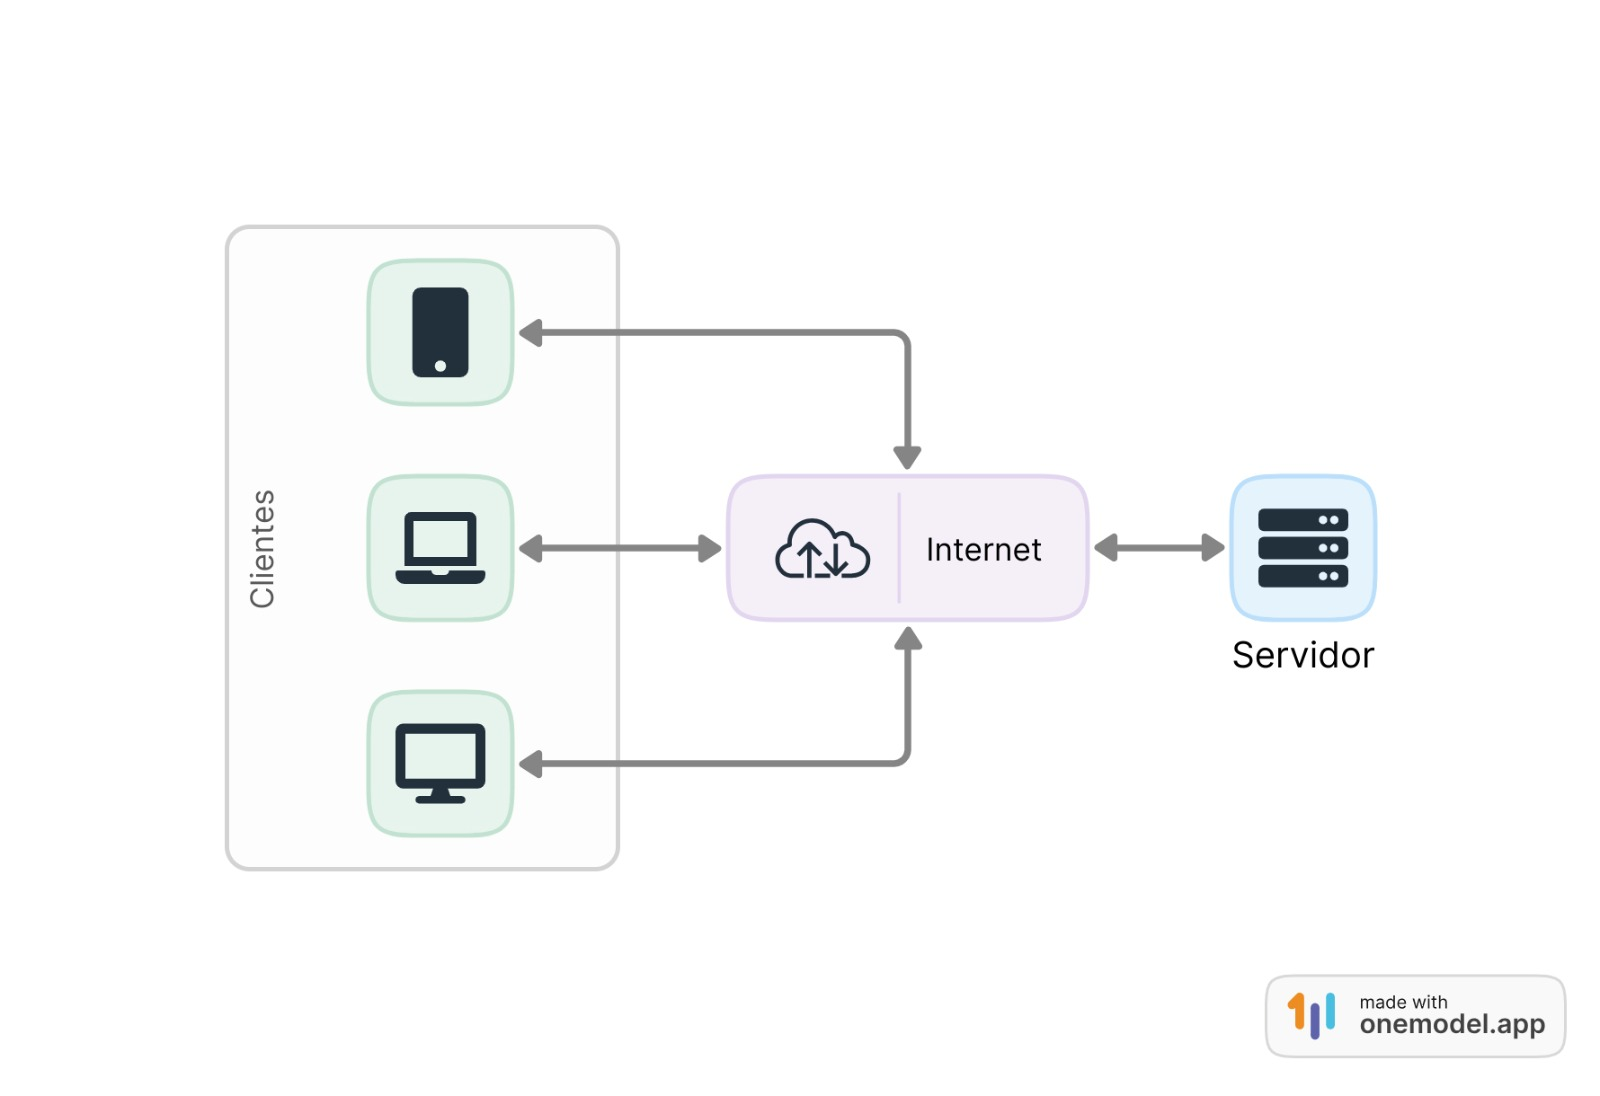
\includegraphics[width=0.8\textwidth]{media/cliente_servidor.jpeg}
  \legend{Fonte: \cite{fundamentosDevWeb} }
  \label{fig:cliente-servidor}
\end{figure}


A arquitetura cliente-servidor apresenta características que contribuem para sua ampla adoção em aplicações web. Entre elas, destaca-se a \textbf{distribuição de responsabilidades}, onde o servidor gerencia dados e processos mais complexos, enquanto o cliente lida com a interface e a interação com o usuário. 

Outro ponto relevante é a \textbf{independência entre plataformas}, possibilitada pelo uso de protocolos padronizados, o que permite a comunicação entre diferentes dispositivos e sistemas operacionais. Além disso, esse modelo favorece a \textbf{facilidade de manutenção}, já que atualizações podem ser feitas no servidor sem necessidade de intervenção nos dispositivos dos usuários.

Na web, essa arquitetura é implementada por padrão: navegadores atuam como clientes, enviando requisições \acrshort{http} que são processadas por servidores, os quais respondem com páginas e recursos solicitados~\cite{fundamentosDevWeb}.


\subsection{Protocolo \acrshort{http}}
\label{subsec:http}
O \textbf{Protocolo de Transferência de Hipertexto} (\acrshort{http}) é a base da comunicação na World Wide Web, definindo como clientes (navegadores) e servidores trocam informações. Ele especifica a estrutura das requisições e respostas, permitindo a recuperação de recursos como documentos \acrshort(html), imagens e vídeos \cite{mdn_http}.


 O \textbf{Funcionamento do \acrshort{http}}opera no modelo cliente-servidor, onde o cliente inicia uma requisição e o servidor responde com os recursos solicitados ou mensagens de erro, se aplicável. Cada interação consiste em uma mensagem de requisição do cliente e uma mensagem de resposta do servidor. As mensagens \acrshort{http} são compostas por:

\begin{itemize}
    \item \textbf{Linha de início:} Indica o método \acrshort{http} (como \texttt{GET} ou \texttt{POST}) e o caminho do recurso.
    \item \textbf{Cabeçalhos:} Fornecem informações adicionais sobre a requisição ou resposta, como tipo de conteúdo e codificação.
    \item \textbf{Corpo:} Contém os dados enviados ou recebidos, sendo opcional dependendo do método utilizado.
\end{itemize}

\begin{flushright}
    \cite{mdn_http}
\end{flushright}


\textbf{Métodos \acrshort{http}} são operações definidas pelo protocolo que especificam a ação a ser realizada em um recurso. Os métodos mais comuns incluem:

\begin{itemize}
    \item \textbf{GET:} Solicita a representação de um recurso específico. Requisições GET devem ser utilizadas apenas para recuperar dados.
    \item \textbf{POST:} Envia dados ao servidor para processamento, como o envio de formulários.
    \item \textbf{PUT:} Atualiza um recurso existente ou cria um novo se não existir.
    \item \textbf{DELETE:} Remove um recurso específico.
    \item \textbf{HEAD:} Similar ao GET, mas solicita apenas os cabeçalhos da resposta, sem o corpo.
\end{itemize}
Cada método possui uma finalidade específica e deve ser utilizado conforme a necessidade da aplicação \cite{wikipedia_http}.


\textbf{Códigos de Status \acrshort{http}} são códigos de três dígitos que indicam o resultado de uma requisição feita pelo cliente ao servidor. Eles são agrupados em cinco classes principais:

\begin{itemize}
    \item \textbf{1xx (Informativo):} Indica que a requisição foi recebida e o processo continua.
    \item \textbf{2xx (Sucesso):} Indica que a requisição foi bem-sucedida. Exemplo: 200 OK.
    \item \textbf{3xx (Redirecionamento):} Indica que é necessário tomar medidas adicionais para completar a requisição. Exemplo: 301 Moved Permanently.
    \item \textbf{4xx (Erro do Cliente):} Indica que houve um erro na requisição do cliente. Exemplo: 404 Not Found.
    \item \textbf{5xx (Erro do Servidor):} Indica que o servidor falhou ao processar uma requisição válida. Exemplo: 500 Internal Server Error.
\end{itemize}

Esses códigos auxiliam na identificação e resolução de problemas durante a comunicação \acrshort{http} \cite{mdn_http}.


\textbf{Evolução do \acrshort{http}} refere-se às revisões progressivas do protocolo com o objetivo de aprimorar sua eficiência e desempenho ao longo do tempo. As principais versões são:

\begin{itemize}
    \item \textbf{HTTP/1.0:} Primeira versão oficial do protocolo, em que cada requisição exigia uma nova conexão com o servidor.
    \item \textbf{HTTP/1.1:} Introduziu conexões persistentes, permitindo múltiplas requisições por conexão. Trouxe também melhorias no controle de cache e suporte a novos métodos.
    \item \textbf{HTTP/2:} Implementou multiplexação, compressão de cabeçalhos e priorização de fluxos, resultando em uma transferência de dados mais rápida e eficiente.
    \item \textbf{HTTP/3:} Baseado no protocolo \acrshort{quic}, substitui o \acrshort{tcp} pelo \acrshort{udp}, oferecendo conexões mais rápidas e seguras, com menor latência e melhor desempenho em redes instáveis.
\end{itemize}

Essas atualizações refletem a evolução das necessidades da web e a busca por protocolos mais robustos e otimizados \cite{cloudflare_http}.

\textbf{\acrshort{http} e \acrshort{https}} representam protocolos utilizados para comunicação na web, com a principal distinção centrada na segurança da transmissão dos dados.

O \textbf{\english{\acrfull{https}}} é uma extensão do \acrshort{http} que adiciona uma camada de proteção por meio do protocolo \english{\acrfull{tls}} ou, anteriormente, \english{\acrfull{ssl}}. Essa camada de segurança garante a confidencialidade, integridade e autenticidade dos dados trafegados entre cliente e servidor. 

A criptografia utilizada impede que terceiros acessem ou modifiquem as informações transmitidas, o que é fundamental em transações sensíveis, como cadastros, pagamentos e autenticações. Além disso, o uso de \textit{certificados digitais} garante que o site visitado é realmente aquele que afirma ser, protegendo os usuários contra ataques como o \textit{man-in-the-middle}\footnote{Um ataque \textit{man-in-the-middle} ocorre quando um invasor intercepta e possivelmente altera a comunicação entre duas partes que acreditam estar se comunicando diretamente. Isso pode permitir que o invasor capture informações sensíveis ou injete dados maliciosos na comunicação.\cite{wikipedia_man_in_the_middle}}.

Enquanto o \acrshort{http} tradicional opera normalmente na porta \acrshort{tcp} 80, o \acrshort{https} utiliza, por convenção, a porta 443. Atualmente, o uso do \acrshort{https} é fortemente recomendado e até exigido por navegadores modernos como padrão de segurança para qualquer aplicação web, contribuindo para a privacidade e confiança dos usuários \cite{wikipedia_http}.

\subsection{\acrshort{html}, \acrshort{css} e JavaScript}
\label{subsec:html-css-js}


O desenvolvimento frontend, conforme definido por \citeonline{aws_frontend_backend}, refere-se à camada de apresentação de uma aplicação web a interface gráfica com a qual os usuários interagem diretamente, composta por menus, botões, formulários e outros elementos visuais. Essa camada baseia-se em um conjunto de tecnologias fundamentais que operam em conjunto para fornecer estrutura, estilo e interatividade às páginas: \acrshort{html}, \acrshort{css} e JavaScript. Cada uma dessas linguagens desempenha um papel específico e complementar, sendo essenciais tanto em abordagens tradicionais quanto em técnicas modernas como o \acrshort{csr}.


\textbf{\acrfull{html}} é a linguagem de marcação padrão para a criação da estrutura de páginas web. Através de um conjunto de elementos (ou \textit{tags}), o \acrshort{html} organiza e define o conteúdo exibido ao usuário, como textos, imagens, links, formulários e tabelas. Além de estruturar visualmente o documento, o \acrshort{html} também confere semântica aos elementos, facilitando a indexação por motores de busca e promovendo acessibilidade para leitores de tela. Elementos como \texttt{<header>}, \texttt{<main>}, \texttt{<article>} e \texttt{<footer>} exemplificam essa função semântica~\cite{alura_htmlcssjs}.

\textbf{\acrfull{css}} é a linguagem responsável pela estilização das páginas web. Com o \acrshort{css}, define-se a aparência dos elementos estruturados no \acrshort{html}, controlando propriedades visuais como cores, fontes, espaçamentos, tamanhos e posicionamentos. O \acrshort{css} permite ainda a construção de layouts complexos e responsivos, adaptando o conteúdo para diferentes tamanhos de tela e dispositivos. A separação entre estrutura (\acrshort{html}) e estilo (\acrshort{css}) é um dos pilares das boas práticas em desenvolvimento web, promovendo manutenibilidade, reutilização e modularidade do código.

Entre os recursos modernos do \acrshort{css}, destacam-se os seletores avançados, variáveis \acrshort{css}, pseudo-classes, animações e as funcionalidades de \textit{Flexbox} e \textit{Grid}, que facilitam a criação de interfaces ricas e adaptáveis~\cite{herocode_diferencas}.

\textbf{JavaScript} é uma linguagem de programação interpretada, orientada a objetos e baseada em eventos, amplamente utilizada para adicionar interatividade e dinamismo às páginas web. Por meio da manipulação da \textit{\acrfull{dom}}, permite implementar funcionalidades como respostas a cliques, envio de formulários, movimentações do mouse, digitação, animações, validações e atualizações em tempo real, enriquecendo significativamente a experiência do usuário~\cite{alura_htmlcssjs}. Além disso, possibilita o carregamento assíncrono de dados com a técnica \textit{AJAX} (\textit{Asynchronous JavaScript and XML}), evitando recarregamentos completos da página.

JavaScript é uma das três principais tecnologias da World Wide Web, juntamente com \acrshort{html} e \acrshort{css}, sendo essencial tanto em abordagens tradicionais quanto modernas. Nas aplicações baseadas em \acrshort{csr}, essa linguagem tem papel central, pois a renderização das páginas ocorre diretamente no navegador do usuário. Com a evolução do ecossistema JavaScript, surgiram bibliotecas e frameworks robustos como a biblioteca React e os frameworks Vue.js e Angular que facilitam o desenvolvimento de aplicações complexas com componentes reutilizáveis e gerenciamento eficiente de estado.

Adicionalmente, o JavaScript também pode ser executado no lado do servidor (\acrshort{ssr}) por meio de ambientes como o Node.js uma plataforma de código aberto e multiplataforma baseada em eventos e não bloqueante, ideal para aplicações escaláveis e em tempo real~\cite{nodejs2025, js2025}. Isso permite o desenvolvimento de aplicações completas utilizando uma única linguagem em ambas as camadas, cliente e servidor.

A interação entre essas três tecnologias pode ser compreendida por meio de uma analogia: o \acrshort{html} representa a estrutura de um corpo (esqueleto), o \acrshort{css} corresponde à sua aparência externa (pele, roupas, estilo), enquanto o JavaScript age como os músculos e o sistema nervoso, controlando os movimentos e respostas interativas da aplicação. A Figura~\ref{fig:html-css-js} ilustra essa relação.

\begin{figure}[H]
  \centering
  \caption{Analogia entre HTML, CSS e JavaScript e os componentes de um corpo humano.}
  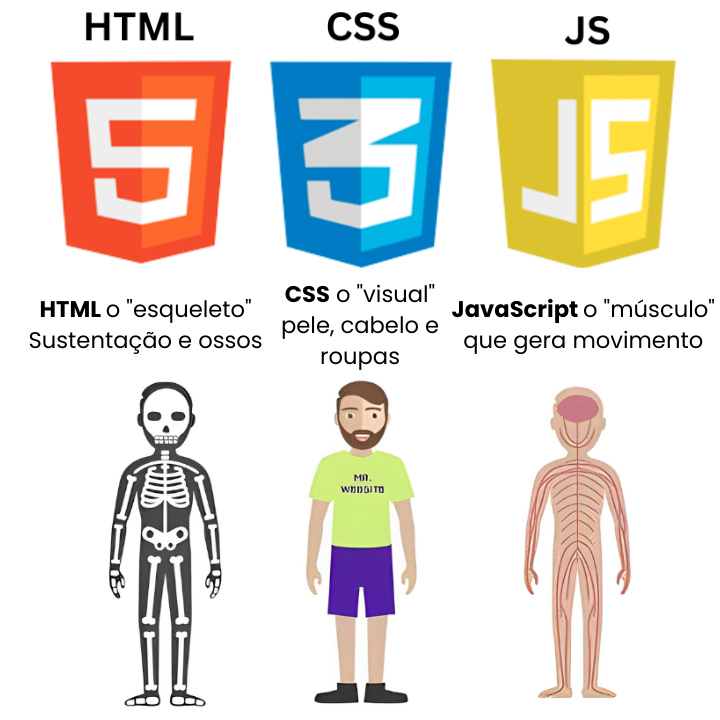
\includegraphics[width=0.6\textwidth]{media/html_css_js_analogia.png}
  \legend{Fonte: \cite{herocode_diferencas}.}
  \label{fig:html-css-js}
\end{figure}

Portanto, o domínio dessas três tecnologias é indispensável para qualquer desenvolvedor web. Elas formam o alicerce sobre o qual se constroem interfaces acessíveis, performáticas e envolventes, sendo empregadas tanto em aplicações renderizadas no servidor (\acrshort{ssr}) quanto no cliente (\acrshort{csr}), com adaptações específicas conforme a abordagem escolhida.



\section{Renderização na Web}
\label{sec:renderizacao-web}

A renderização na Web diz respeito ao processo de transformar dados em conteúdo visual interpretável pelo navegador. A escolha sobre onde e como essa renderização será realizada (seja no cliente, no servidor ou em tempo de build), isso impacta diretamente métricas como tempo de carregamento, interatividade e indexação por mecanismos de busca \cite{osmani2025}.


\subsection{\acrfull{spa} e \acrfull{mpa}}
\label{subsec:spa-mpa}

As arquiteturas \acrfull{spa} e \acrfull{mpa} representam duas abordagens distintas para a estrutura de navegação e carregamento de conteúdo em aplicações web.

As \acrshort{spa}s são aplicações em que a navegação entre páginas ocorre sem recarregamentos completos do navegador. Após o carregamento inicial, todo o conteúdo adicional é gerenciado dinamicamente com JavaScript, o que proporciona uma experiência mais fluida e interativa. Essa abordagem é comumente utilizada em conjunto com a renderização no lado do cliente (\acrshort{csr}) e frameworks como React, Angular ou Vue.js \cite{atori2024}.

Já as \acrshort{mpa}s seguem o modelo tradicional de navegação, em que cada clique em um link leva a uma nova requisição \acrshort{http} e recarregamento completo da página. Essa arquitetura é naturalmente mais compatível com a renderização no lado do servidor (\acrshort{ssr}) e favorece aspectos como \acrshort{seo}, acessibilidade e previsibilidade de comportamento \cite{osmani2025}.

A escolha entre \acrshort{spa} e \acrshort{mpa} está diretamente ligada à estratégia de renderização adotada. As \acrshort{spa}s tendem a oferecer experiências mais ricas e responsivas, mas exigem cuidados extras com desempenho e indexação. Por outro lado, as \acrshort{mpa}s são mais robustas em cenários com grande volume de tráfego e requisitos de otimização para mecanismos de busca.



\subsection*{Conceitos e Terminologia}

Segundo \citeonline{osmani2025}, é importante distinguir os principais modelos:


\begin{description}
  \item[\textbf{Client-Side Rendering (CSR)}] 
  O conteúdo da aplicação é gerado dinamicamente no navegador, utilizando JavaScript. A página HTML inicial contém apenas uma estrutura básica com os scripts necessários para montar a interface após o carregamento. É comum em aplicações do tipo SPA (Single Page Application).
  
  \item[\textbf{Server-Side Rendering (SSR)}]
  O servidor monta todo o conteúdo da página em HTML antes de enviá-lo ao cliente. Isso permite uma exibição mais rápida do conteúdo, mesmo em conexões lentas, e melhora a indexação por mecanismos de busca.

  \item[\textbf{Static Site Generation (SSG)}]
  As páginas são geradas de forma estática em tempo de build, com base em dados disponíveis no momento da compilação. O conteúdo é entregue diretamente por uma CDN, garantindo alto desempenho.

  \item[\textbf{Incremental Static Regeneration (ISR)}]
  Introduzido pelo Next.js, o ISR permite que páginas geradas estaticamente possam ser atualizadas de forma incremental, após um período de tempo definido. Isso é feito em segundo plano, sem bloquear o carregamento da página atual. Ideal para sites com atualizações frequentes, mas não críticas em tempo real.

  \item[\textbf{Deferred Static Generation (DSG)}]
  Proposto pelo Gatsby, o DSG difere do ISR por não gerar certas páginas no momento do build. Em vez disso, elas são geradas apenas na primeira requisição (on-demand). Após isso, são armazenadas em cache e servidas como estáticas nas requisições seguintes. É útil em projetos com milhares de páginas de baixo acesso, reduzindo significativamente o tempo de build.
\end{description}

Além dessas abordagens, destaca-se o conceito de \textbf{reidratação}, que consiste em ativar a interatividade de páginas SSR ou SSG no cliente. Esse processo utiliza JavaScript para associar os eventos dinâmicos à estrutura HTML previamente renderizada, sendo essencial para tornar a página interativa após a exibição inicial \cite{osmani2025}.


Esses métodos influenciam diretamente métricas como:

\begin{itemize}
    \item \textbf{TTFB (Time to First Byte)}: tempo até o primeiro byte da resposta.
    \item \textbf{FCP (First Contentful Paint)}: quando o conteúdo começa a ser exibido.
    \item \textbf{TTI (Time to Interactive)}: quando a página se torna responsiva.
    \item \textbf{INP (Interaction to Next Paint)} e \textbf{TBT (Total Blocking Time)}: indicadores de interatividade e bloqueio da thread principal.
\end{itemize}

\subsection*{Desempenho e Compensações}

A renderização do lado do servidor tende a exibir conteúdo mais rapidamente (menor FCP), favorecendo acessibilidade e \textit{SEO}. No entanto, pode aumentar o TTFB, já que a página precisa ser processada antes de ser enviada \cite{osmani2025}. Já a renderização no cliente pode reduzir o tempo de resposta inicial do servidor, mas exige mais do navegador e aumenta o tempo até a página estar interativa (TTI), especialmente em dispositivos móveis.

Modelos híbridos como SSR com \textit{hydration} tentam unir os benefícios de ambas as abordagens, mas podem causar atrasos na interatividade. Técnicas como \textit{hydration progressiva} ou \textit{streaming} reduzem esses impactos ao ativar partes da interface conforme necessário \cite{osmani2025}.

\subsection*{Avanços Recentes}

Estratégias mais recentes, como a \textbf{renderização trimórfica}, permitem que a renderização ocorra em três camadas: servidor, cliente e \textit{service worker}. Isso possibilita desempenho superior em acessos repetidos e melhor controle sobre o cache e atualização de conteúdo dinâmico \cite{osmani2025}.

\subsection*{Impacto em SEO e Indexação}

Segundo \citeonline{osmani2025}, abordagens que entregam HTML completo como SSR e SSG são mais eficazes para indexação por mecanismos de busca. Já modelos que dependem fortemente de JavaScript (CSR) exigem testes adicionais e podem comprometer a visibilidade em sistemas como o Googlebot, especialmente quando há falhas na execução dos scripts.

\begin{figure}[H]
  \centering
  \caption{Comparativo entre estratégias de renderização}
  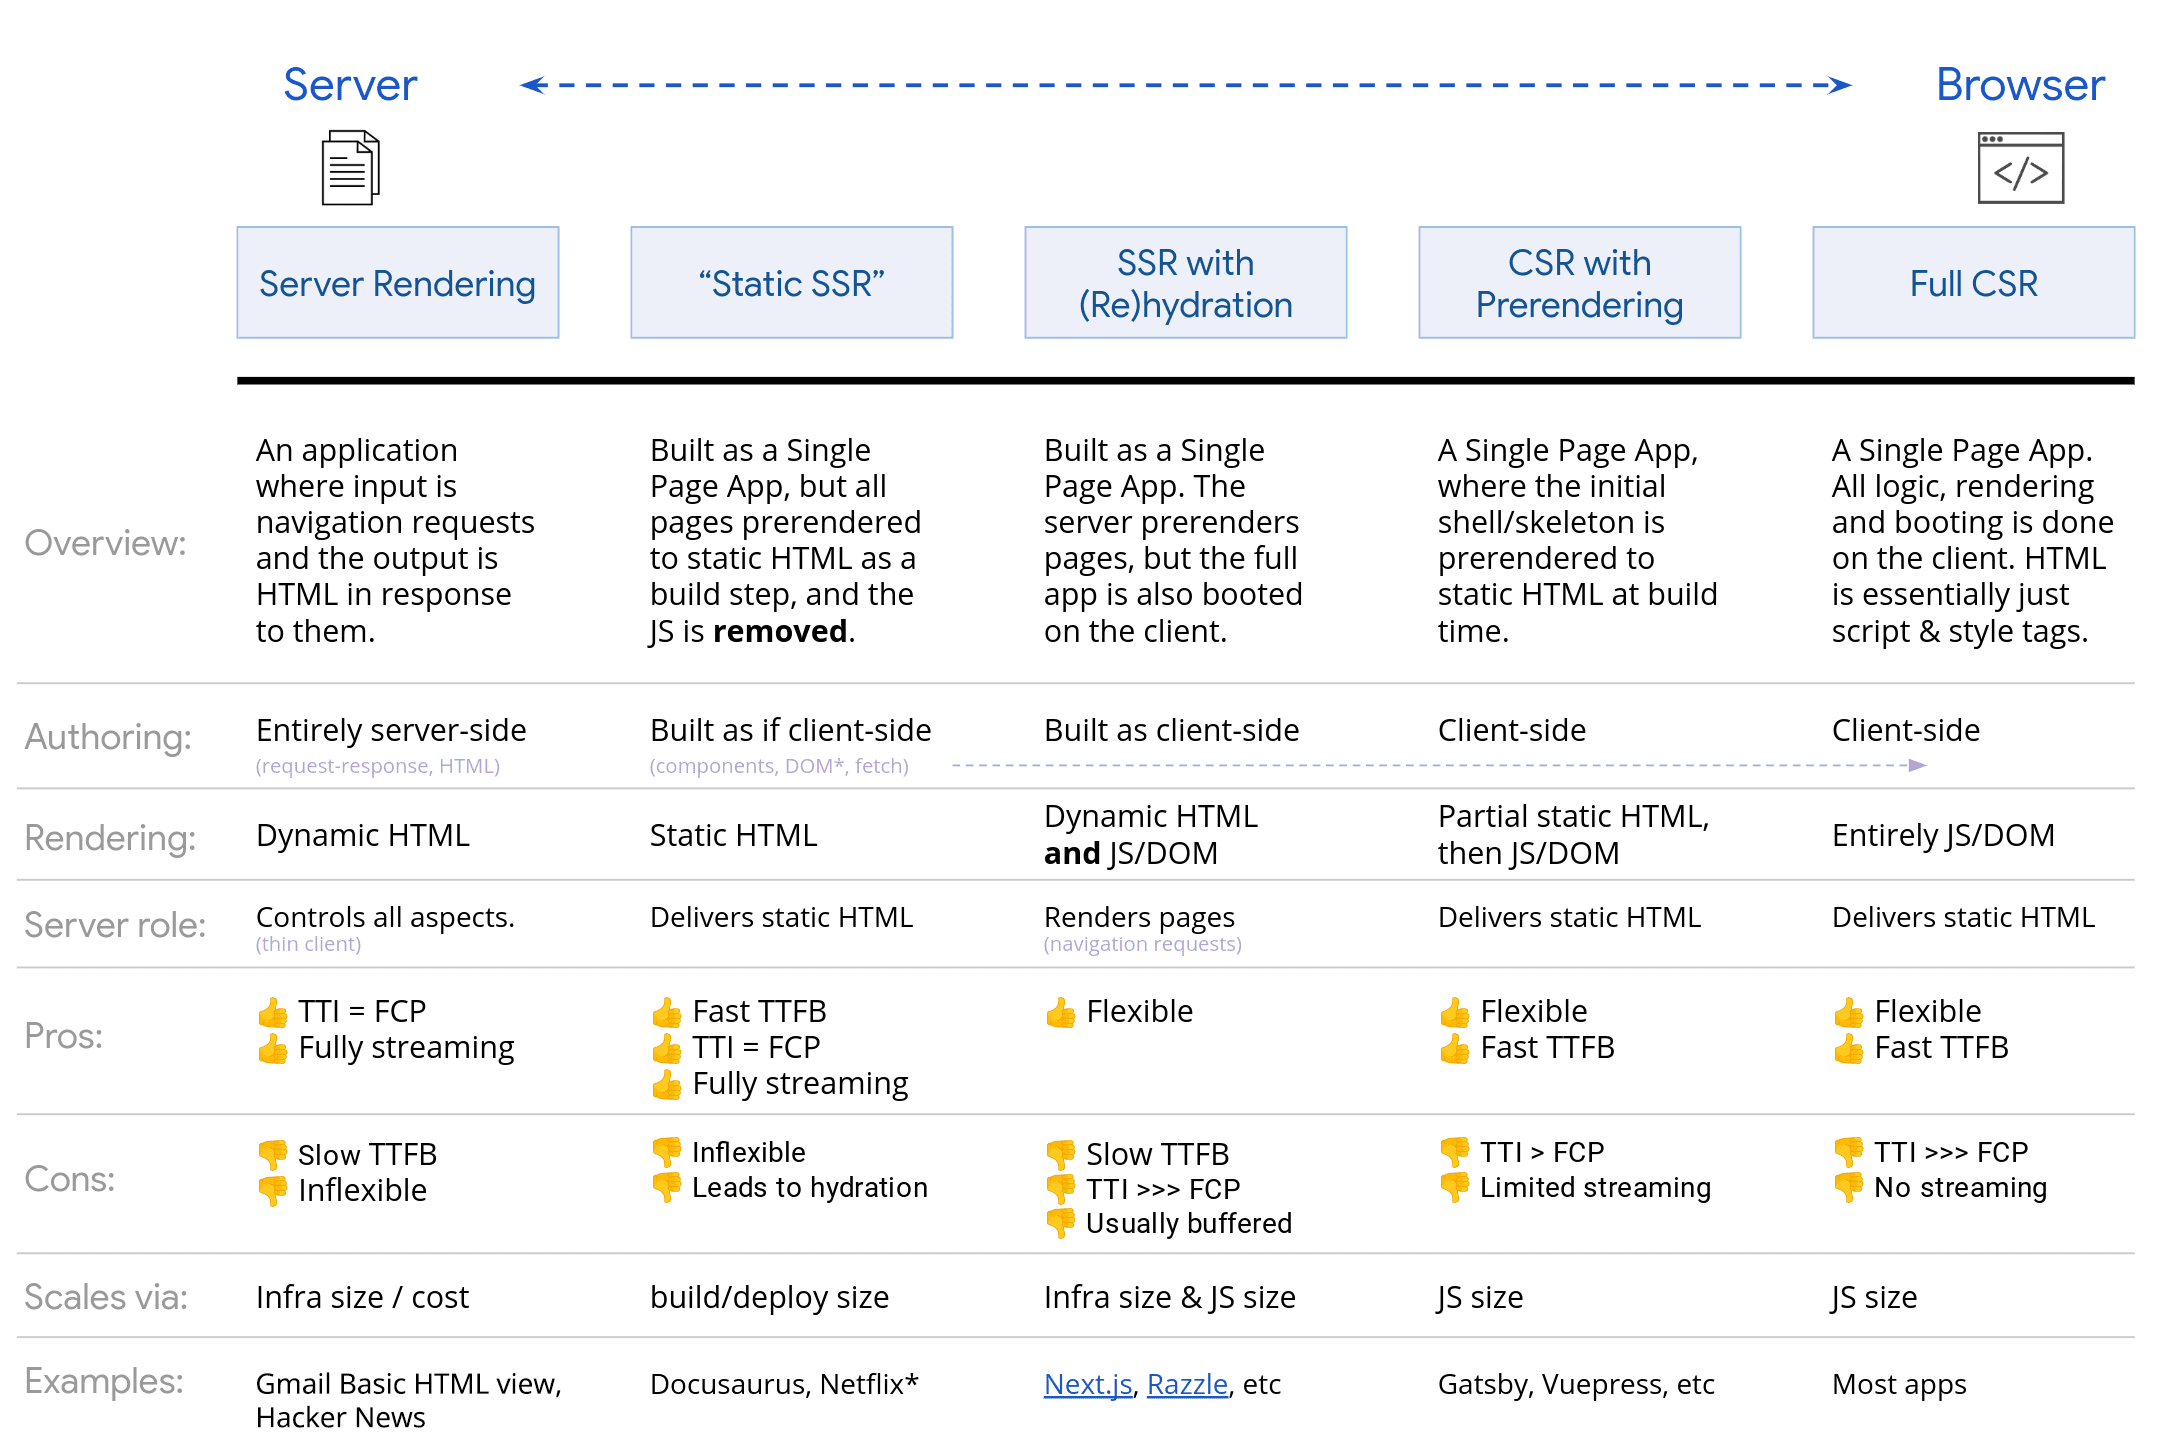
\includegraphics[width=\textwidth]{media/rendering_comparison_table.png}
  \legend{Fonte: Adaptado de \cite{osmani2025}}
  \label{fig:comparativo_renderizacao}
\end{figure}



\subsection{\english{Client-Side Rendering} (\acrshort{csr})}
\label{subsec:csr}

A \textbf{\english{\acrfull{csr}}} é uma técnica em que a geração da interface e do conteúdo final ocorre diretamente no navegador do usuário, utilizando JavaScript. Nessa abordagem, o servidor envia um arquivo \english{\acrfull{html}} mínimo, contendo apenas a estrutura básica da página e referências a arquivos de estilo e scripts.{\cite{atori2024}}

Segundo \citeonline{atori2024}, o processo de renderização no cliente segue as seguintes etapas:

\begin{enumerate}
    \item O servidor envia uma página \acrshort{html} em branco contendo apenas links para os arquivos \english{\acrfull{css}} e JavaScript.
    \item O navegador interpreta o \acrshort{html} e constrói a árvore do \english{\acrfull{dom}}
    \item Os arquivos de estilo (\acrshort{css}) e script (JavaScript) são baixados pelo navegador.
    \item A aplicação é renderizada dinamicamente pelo JavaScript, incluindo elementos visuais como texto, imagens e botões.
    \item O conteúdo da página é atualizado de forma interativa conforme o usuário interage com a aplicação.
\end{enumerate}

Esse modelo é comumente utilizado em aplicações \english{\acrfull{spa}}, nas quais o carregamento inicial é seguido por atualizações dinâmicas sem recarregamento da página. Ferramentas como a biblioteca React, e frameworks como Vue.js, Angular e Svelte são amplamente utilizadas para implementar \acrshort{csr}, permitindo o desenvolvimento de interfaces dinâmicas, interativas e responsivas.


A renderização no lado do cliente (\acrshort{csr}) é especialmente vantajosa em aplicações que exigem alta interatividade e atualizações frequentes de conteúdo, como redes sociais, plataformas de streaming e jogos online. No entanto, essa abordagem pode apresentar desvantagens em termos de desempenho inicial e \acrshort{seo}, uma vez que o conteúdo só é exibido após a execução do JavaScript, o que pode impactar negativamente a indexação por motores de busca e a experiência do usuário em conexões lentas \cite{atori2024}.

\begin{figure}[h!]
    \centering
    \caption{Etapas do método de renderização no lado do cliente}
    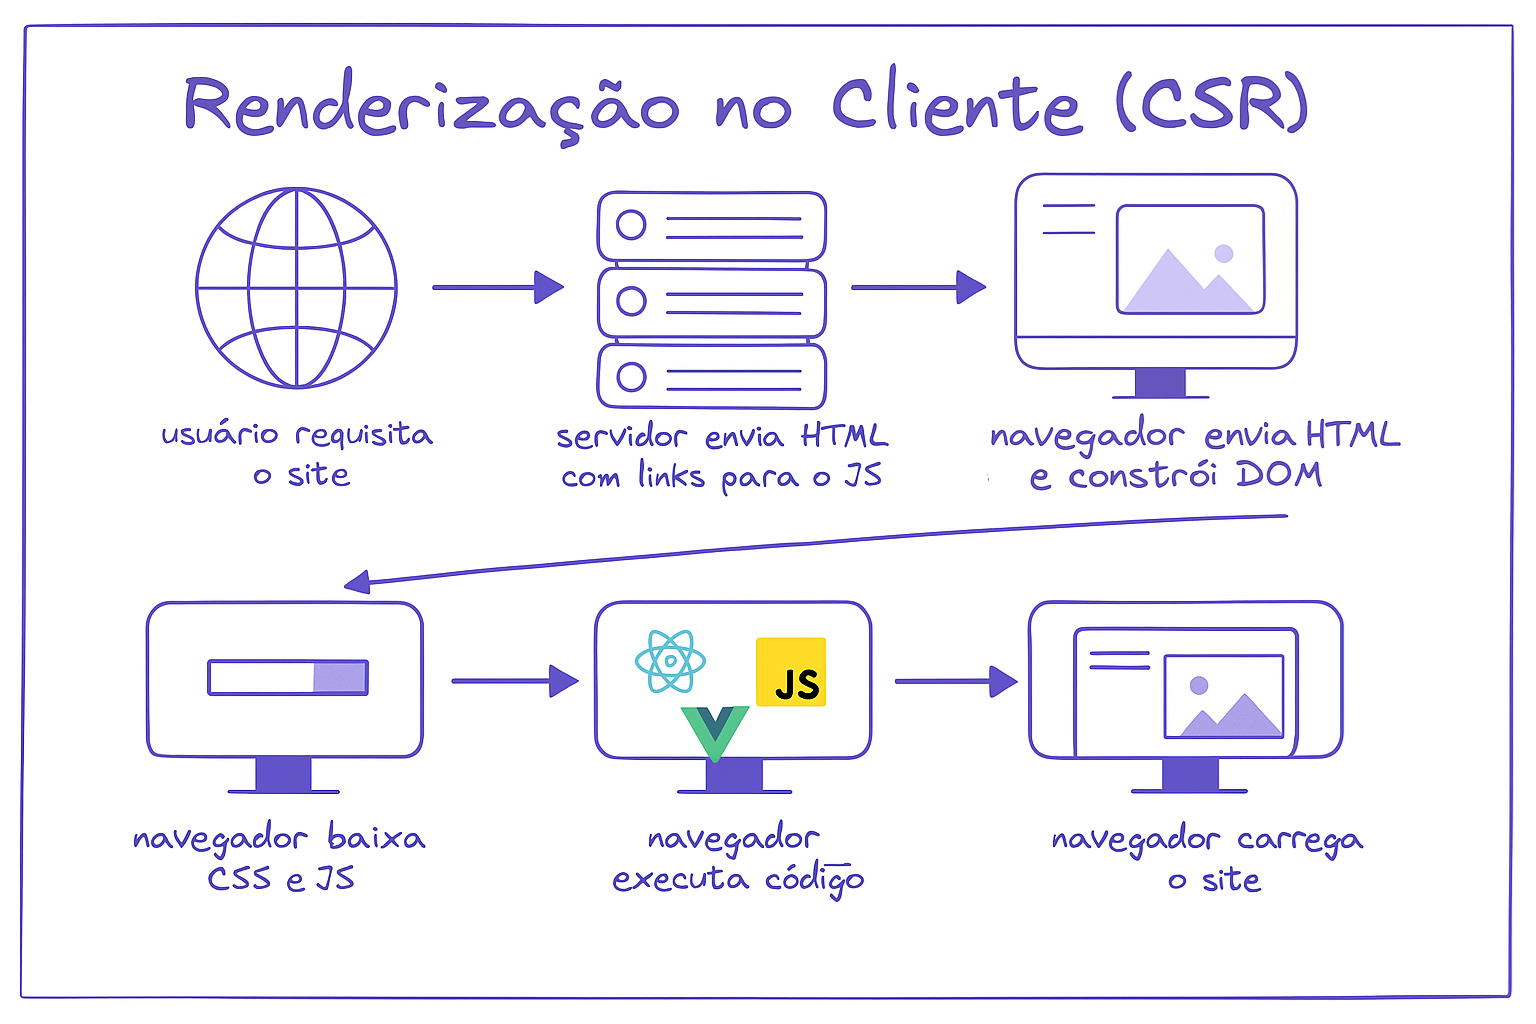
\includegraphics[width=0.8\textwidth]{media/client_side_rendering.png}
    \legend{Fonte: \cite{atori2024} (adaptado)}
    \label{fig:client_side_rendering}
\end{figure}


A \autoref{fig:client_side_rendering} ilustra visualmente o fluxo completo da renderização no lado do cliente (\acrshort{csr}). O processo é iniciado quando o usuário acessa o site em questão. Em resposta, o servidor envia o arquivo \acrshort{html} básico, contendo apenas links para os arquivos de estilo \acrshort{css} e scripts JavaScript responsáveis por carregar e renderizar o conteúdo da aplicação.

Na sequência, o navegador interpreta esse \acrshort{html} e constrói a estrutura da página por meio da árvore \acrshort{dom}. No entanto, o conteúdo principal ainda não está visível. O navegador então precisa baixar os arquivos de estilo (\acrshort{css}) e os scripts JavaScript referenciados no documento inicial.

Com os scripts carregados, o navegador executa o código JavaScript, que normalmente utiliza bibliotecas ou frameworks como React ou Vue para gerar dinamicamente o conteúdo da aplicação. Somente após essa etapa o conteúdo completo do site é finalmente exibido ao usuário, quando o navegador conclui o processo de renderização e o site é carregado completamente.

\begin{codigo}[H]
  \begin{lstlisting}[language=html]
<!DOCTYPE html>
<html lang="en">
<head>
  <meta charset="utf-8">
  <title>CryptoWebsite</title>
  <base href="/">
  <meta name="viewport" content="width=device-width, initial-scale=1">
  <link rel="icon" type="image/x-icon" href="favicon.ico">
  <style>*,*:before,*:after{margin:0;padding:0;box-sizing:border-box;
    font-family:Inter,sans-serif}html{font-size:62.5%}</style>
  <link rel="stylesheet" href="styles.9d4c7581c7242.css">
</head>
<body>
  <app-root></app-root>
  <script src="runtime.6170988ad52a05db.js" type="module"></script>
  <script src="polyfills.574970d5ec4bdb97.js" type="module"></script>
  <script src="main.202d37bb6740400e.js" type="module"></script>
</body>
</html>
\end{lstlisting}
  \caption{Exemplo de HTML mínimo em aplicação Angular com CSR}
  \label{lst:angular_html}
\end{codigo}

Esse padrão é típico de aplicações \acrshort{spa}, onde todo o conteúdo é inserido dinamicamente a partir da execução dos arquivos JavaScript. O elemento \texttt{<app-root>} funciona como ponto de entrada da aplicação, sendo substituído no navegador pelos componentes definidos no framework Angular. {\cite{atori2024}}


\subsection{\english{Server-Side Rendering} (\acrshort{ssr})}
\label{subsec:ssr}

A \textbf{\english{\acrfull{ssr}}} é uma abordagem em que a geração do conteúdo e da interface ocorre integralmente no servidor antes de ser enviada ao navegador do cliente. Ou seja, o servidor processa a lógica da aplicação, obtém dados necessários (por exemplo, em bancos de dados ou \emph{APIs}) e retorna ao cliente um arquivo \english{\acrshort{html}} já renderizado. Dessa forma, o navegador exibe imediatamente a página completa, sem precisar executar \emph{scripts} para montar o conteúdo inicial \cite{atori2024}. 

Segundo \citeonline{atori2024}, o processo típico de renderização no lado do servidor pode ser descrito em quatro etapas principais:

\begin{enumerate}
    \item O servidor recebe uma requisição para uma página e recupera os dados necessários para compor seu conteúdo (por exemplo, produtos de uma base de dados ou artigos de um blog).
    \item O servidor insere esses dados em um \emph{template} \acrshort{html}, gerando a estrutura final da página.
    \item Em seguida, o servidor aplica estilos e finaliza a renderização, resultando em um documento \acrshort{html} completamente montado.
    \item Por fim, esse documento \acrshort{html} é enviado ao navegador do usuário, exibindo a página prontamente, sem a necessidade de executar \emph{JavaScript} durante o carregamento inicial.
\end{enumerate}

Nesse modelo, a fase de hydration\footnote{Hydration é uma etapa essencial no \acrshort{ssr}, em que o JavaScript torna interativo o conteúdo HTML previamente renderizado no servidor.} ocorre após o carregamento inicial da página. costuma ocorrer após a entrega do conteúdo estático. Significa que, assim que o arquivo \acrshort{html} é carregado e mostrado ao usuário, o \emph{JavaScript} do lado do cliente assume o controle para tratar as interações e atualizações dinâmicas subsequentes. Dessa forma, o \acrshort{ssr} beneficia tanto o primeiro acesso (tornando o conteúdo visível rapidamente) quanto o \acrshort{seo}, por exibir ao rastreador dos mecanismos de busca um código \acrshort{html} completo. \cite{atori2024}.

\begin{figure}[H]
  \centering
  \caption{Etapas do método de renderização no lado do servidor}
  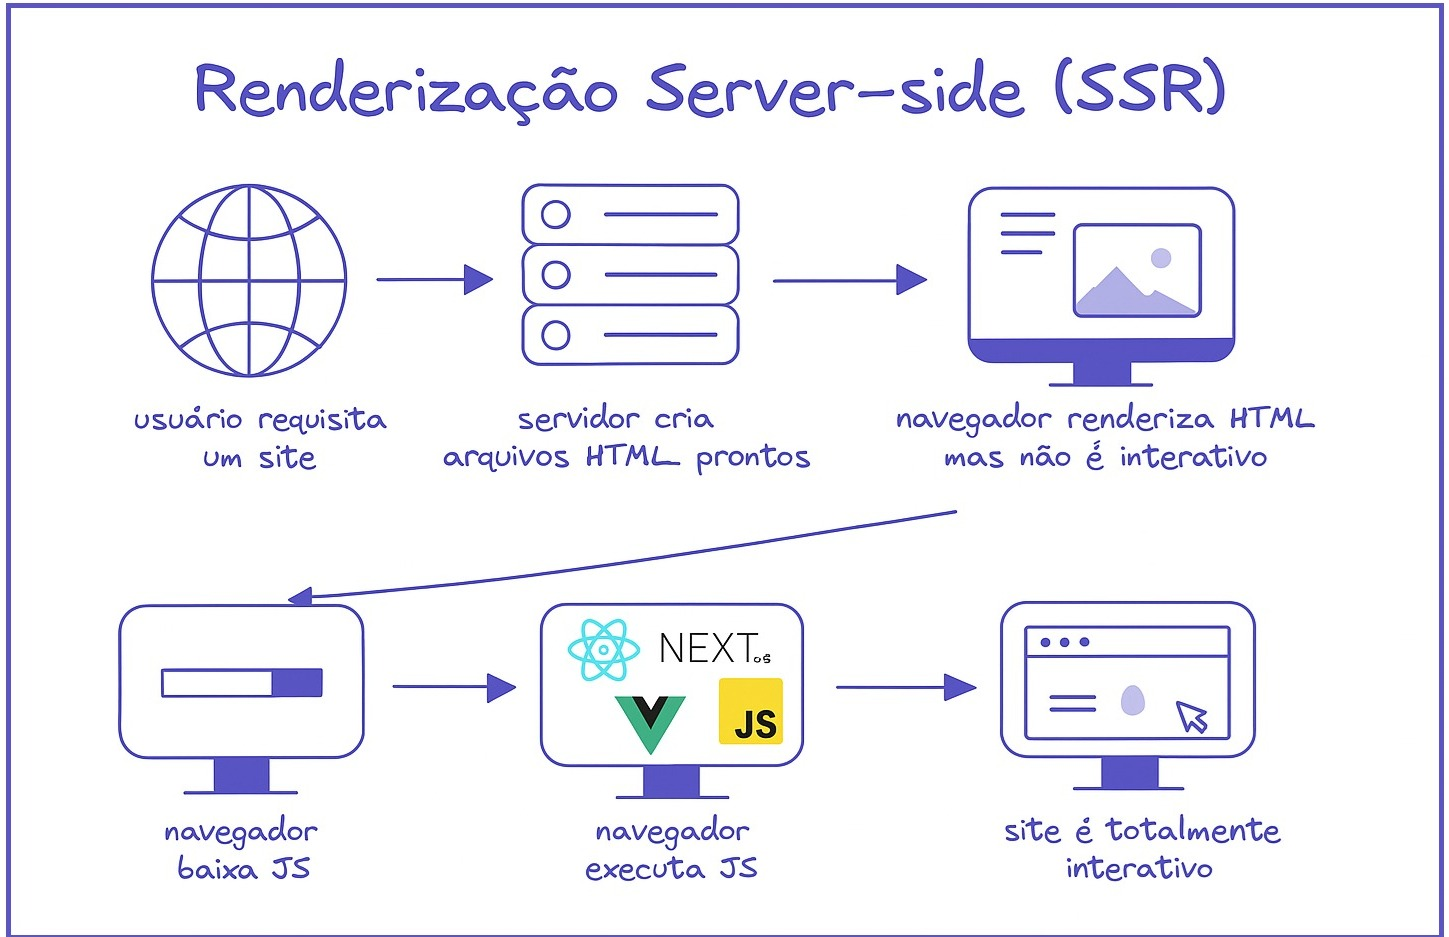
\includegraphics[width=0.8\textwidth]{media/server_side_rendering.jpeg}
  \legend{Fonte: \cite{atori2024} (adaptado)}
  \label{fig:server_side_rendering}
\end{figure}

A \autoref{fig:server_side_rendering} ilustra o fluxo de uma aplicação \acrshort{ssr}. Ao receber a requisição, o servidor gera a página completa em \acrshort{html} e a envia ao cliente. Essa estratégia costuma ser vantajosa em cenários onde o carregamento inicial rápido e a indexação por motores de busca são prioridades, como em sites de e-commerce e páginas de \emph{landing}, permitindo que o usuário visualize o conteúdo de forma imediata. 

\emph{Meta-frameworks} como Next.js, Nuxt.js, SvelteKit, Angular Universal, Remix, Astro e Qwik são amplamente utilizados para construir aplicações com suporte a \acrshort{ssr}. Esses frameworks operam em um nível superior aos tradicionais (como React, Vue ou Svelte), agregando funcionalidades comuns ao desenvolvimento web, como roteamento, pré-renderização, recuperação de dados e \emph{hydration} podendo oferecer uma estrutura mais completa, opinativa e voltada à escalabilidade.

O \acrshort{ssr} é especialmente útil em aplicações que exigem um carregamento inicial rápido e uma boa indexação por motores de busca, como sites de e-commerce, blogs e páginas de \emph{landing}. Essa abordagem permite que o usuário visualize o conteúdo imediatamente, sem esperar pela execução do JavaScript. Além disso, o \acrshort{ssr} melhora a \acrshort{seo}, pois os mecanismos de busca conseguem indexar o conteúdo completo da página desde o início.

No \autoref{cod:nextjs_html}, pode-se observar que o arquivo \acrshort{html} já contém todo o \emph{markup} necessário para exibir o conteúdo da página. Assim que o navegador recebe esse arquivo, o usuário já visualiza o cabeçalho, o texto e o layout definidos. Posteriormente, o \emph{JavaScript} baixado (por exemplo, \texttt{main.js}) pode entrar em ação para lidar com eventos, rotas adicionais e atualizações dinâmicas, caso o desenvolvedor deseje funcionalidades mais interativas.

Por fim, aplicações \acrshort{ssr} tendem a apresentar melhor performance em termos de \emph{time-to-first-byte}\footnote{O \emph{time-to-first-byte} (TTFB) é uma métrica que mede o tempo decorrido entre o envio de uma solicitação HTTP pelo cliente e o recebimento do primeiro byte da resposta do servidor. Um TTFB menor indica maior rapidez na resposta do servidor, impactando diretamente na velocidade de carregamento da página e na experiência do usuário. \cite{ttfb-craig}} e de \emph{indexabilidade}\footnote{A \emph{indexabilidade} refere-se à capacidade dos motores de busca de rastrear e indexar o conteúdo de uma página web. Aplicações SSR, ao fornecerem conteúdo totalmente renderizado no servidor, facilitam a indexação eficiente pelos motores de busca, melhorando a visibilidade nos resultados de pesquisa. \cite{ttfb-oskay}} por motores de busca, ao mesmo tempo em que podem demandar maior carga de processamento no servidor. A escolha por \acrshort{ssr} ou não, portanto, depende do perfil da aplicação e das prioridades do projeto, considerando fatores como volume de tráfego, necessidade de interatividade e requisitos de otimização de conteúdo.

\begin{codigo}[H]
  \begin{lstlisting}[language=html]
    <!DOCTYPE html>
    <html lang="en">
    <head>
      <meta charset="utf-8">
      <title>My SSR App</title>
      <meta name="viewport" content="width=device-width, initial-scale=1">
      <style>
        /* Exemplo simples de estilo inline */
        body {
          margin: 0;
          font-family: Arial, sans-serif;
          background: #f6f6f6;
        }
        h1 { color: #333; }
      </style>
    </head>
    <body>
<!-- Conteudo ja processado e inserido no servidor -->
      <div id="__next">
        <header>
          <h1>Ola, mundo!</h1>
        </header>
        <main>
          <p>Este conteudo foi renderizado no servidor usando Next.js.</p>
        </main>
      </div>
      <!-- Scripts do Next.js para interacao no cliente -->
      <script src="/_next/static/chunks/main.js" defer></script>
    </body>
    </html>
  \end{lstlisting}
  \caption{Exemplo de HTML mínimo em aplicação Next.js com SSR}
  \label{cod:nextjs_html}
\end{codigo}

\subsection{\english{Static Site Generation} (\acrshort{ssg})}
\label{subsec:ssg}

A \textbf{\english{\acrfull{ssg}}} é uma técnica de pré-renderização na qual as páginas da aplicação são geradas estaticamente em tempo de *build* (compilação) e armazenadas como arquivos \acrshort{html}. Ao contrário de abordagens como \acrshort{csr} e \acrshort{ssr}, onde a renderização ocorre no navegador ou sob demanda no servidor, o \acrshort{ssg} permite que o conteúdo já esteja pronto e otimizado para ser entregue diretamente ao navegador, reduzindo a carga do servidor e otimizando o desempenho de carregamento \cite{pahan2021}.

Segundo \citeonline{bose2022}, a renderização no modelo \acrshort{ssg} segue estas etapas principais:

\begin{enumerate}
    \item Durante o processo de construção (build), o gerador de sites estáticos coleta dados de fontes como arquivos locais, \emph{APIs} ou bancos de dados.
    \item Esses dados são utilizados para gerar arquivos \acrshort{html} completos para cada rota da aplicação.
    \item Os arquivos gerados são armazenados e podem ser servidos diretamente por uma \emph{CDN} (Content Delivery Network).
    \item Quando o usuário acessa a aplicação, os arquivos estáticos são entregues instantaneamente, sem necessidade de renderização adicional.
\end{enumerate}

Essa abordagem é ideal para páginas cujo conteúdo não muda com frequência, como blogs, documentações, portfólios e sites institucionais. Como os arquivos são pré-gerados, o tempo de resposta é extremamente rápido, e o \acrshort{seo} é favorecido, já que os mecanismos de busca encontram o conteúdo pronto para indexação.

\begin{figure}[H]
  \centering
  \caption{Etapas do método de geração estática de páginas (SSG)}
  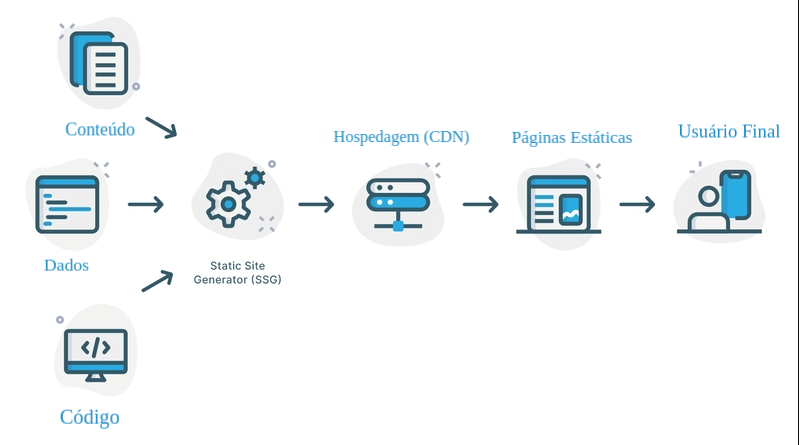
\includegraphics[width=0.8\textwidth]{media/static_site_generation.png}
  \legend{Fonte: \cite{bose2022} (adaptado)}
  \label{fig:ssg}
\end{figure}

Frameworks como Next.js, Gatsby, Hugo e Jekyll oferecem suporte completo ao \acrshort{ssg}, integrando funcionalidades como roteamento dinâmico, \emph{markdown}, e integração com CMSs. No exemplo a seguir, observa-se um documento \acrshort{html} gerado estaticamente por meio de um processo de \emph{build}:

\begin{codigo}[H]
  \begin{lstlisting}[language=html]
<!DOCTYPE html>
<html lang="en">
  <head>
    <meta charset="UTF-8" />
    <meta name="viewport" content="width=device-width, initial-scale=1.0" />
    <title>Post: SSG Example</title>
  </head>
  <body>
    <article>
      <h1>Exemplo de página gerada com SSG</h1>
      <p>Esse conteúdo foi gerado em tempo de build.</p>
    </article>
  </body>
</html>
  \end{lstlisting}
  \caption{Exemplo de HTML estático gerado com SSG}
  \label{cod:ssg_example}
\end{codigo}

A principal limitação do \acrshort{ssg} é a dificuldade em lidar com conteúdos altamente dinâmicos. Alterações nos dados requerem um novo processo de build para que as páginas sejam atualizadas, o que pode ser custoso em grandes aplicações ou com frequência de atualização elevada.

\subsection{\english{Incremental Static Regeneration} (\acrshort{isr})}
\label{subsec:isr}

A \textbf{\english{\acrfull{isr}}} é uma estratégia híbrida introduzida por frameworks como o Next.js, que combina os benefícios da geração estática (\acrshort{ssg}) com a flexibilidade de atualização dinâmica. Com \acrshort{isr}, as páginas são inicialmente geradas estaticamente em tempo de build, mas podem ser revalidadas e regeneradas no servidor de forma incremental e automática, com base em uma estratégia de tempo (ex: a cada 10 segundos) ou conforme novas requisições são feitas \cite{pahan2021}.

De acordo com \citeonline{bose2022}, o fluxo típico do \acrshort{isr} inclui as seguintes etapas:

\begin{enumerate}
    \item No momento do build inicial, as páginas são geradas e armazenadas como arquivos estáticos.
    \item Ao ser requisitada por um usuário, a página é entregue imediatamente, com o conteúdo pré-renderizado.
    \item Se o tempo de revalidação definido (ex: \texttt{revalidate: 60}) tiver expirado, uma nova requisição ao backend é feita em segundo plano.
    \item Essa nova versão da página é armazenada e substitui a anterior, sendo usada em acessos futuros.
\end{enumerate}

Essa abordagem permite obter performance e \acrshort{seo} semelhantes ao \acrshort{ssg}, mas com a vantagem de manter o conteúdo atualizado sem precisar de reconstruções manuais. Por isso, o \acrshort{isr} é ideal para sites que possuem atualizações regulares, porém não críticas em tempo real, como catálogos de produtos, blogs com comentários ou páginas de notícias.

\begin{figure}[H]
  \centering
  \caption{Funcionamento do modelo Incremental Static Regeneration (ISR)}
  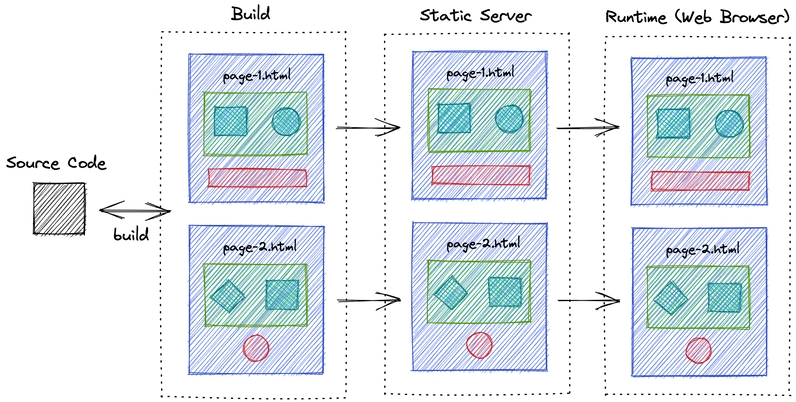
\includegraphics[width=0.8\textwidth]{media/incremental_static_regeneration.png}
  \legend{Fonte: \cite{pahan2021}}
  \label{fig:isr}
\end{figure}

Abaixo, um exemplo típico em Next.js:

\begin{codigo}[H]
  \begin{lstlisting}[language=JavaScript]
      // Funcao usada em getStaticProps
      export async function getStaticProps() {
        const res = await fetch('https://api.exemplo.com/posts')
        const posts = await res.json()

        return {
          props: { posts },
          revalidate: 60, // Pagina sera regenerada a cada 60 segundos
          }
      }
  \end{lstlisting}
  \caption{Exemplo de revalidação de conteúdo com ISR no Next.js}
  \label{cod:isr_next}
\end{codigo}


O \acrshort{isr} representa um meio-termo eficiente entre a performance do \acrshort{ssg} e a flexibilidade do \acrshort{ssr}, oferecendo escalabilidade, \acrshort{seo} eficiente e atualização contínua do conteúdo, sem prejudicar a experiência do usuário.




\subsection{\english{Deferred Static Generation} (\acrshort{dsg})}
\label{subsec:deferred-dsg}

A \textbf{\english{Deferred Static Generation} (DSG)} é uma extensão da estratégia de geração estática proposta pelo framework Gatsby. Essa abordagem permite que certas páginas do site sejam geradas sob demanda ( ou seja, somente no momento em que forem requisitadas pela primeira vez ) em vez de serem construídas durante o processo inicial de build, como ocorre no \acrshort{ssg} tradicional \cite{gatsby2023}.

Segundo a \citeonline{gatsby2023}, o \acrshort{dsg} tem como principal vantagem a capacidade de reduzir significativamente o tempo de build em projetos com um número elevado de páginas, ao evitar a pré-renderização de rotas que têm baixo tráfego ou que não precisam estar imediatamente disponíveis. Após a primeira solicitação, a página é armazenada em cache e, a partir daí, servida como conteúdo estático em acessos subsequentes.

O fluxo típico de geração diferida no \acrshort{dsg} ocorre da seguinte forma:

\begin{enumerate}
    \item Durante o processo de build, apenas páginas prioritárias são pré-geradas.
    \item Páginas marcadas como \texttt{defer} são ignoradas temporariamente.
    \item Quando uma página \acrshort{dsg} é acessada pela primeira vez, um \textit{worker} do Gatsby gera a versão \acrshort{html} da página com base em um componente React (ex: \texttt{about.js}).
    \item A página gerada é armazenada em cache e servida como conteúdo estático nas próximas requisições.
\end{enumerate}

\begin{figure}[H]
  \centering
  \caption{Funcionamento da estratégia Deferred Static Generation (DSG)}
  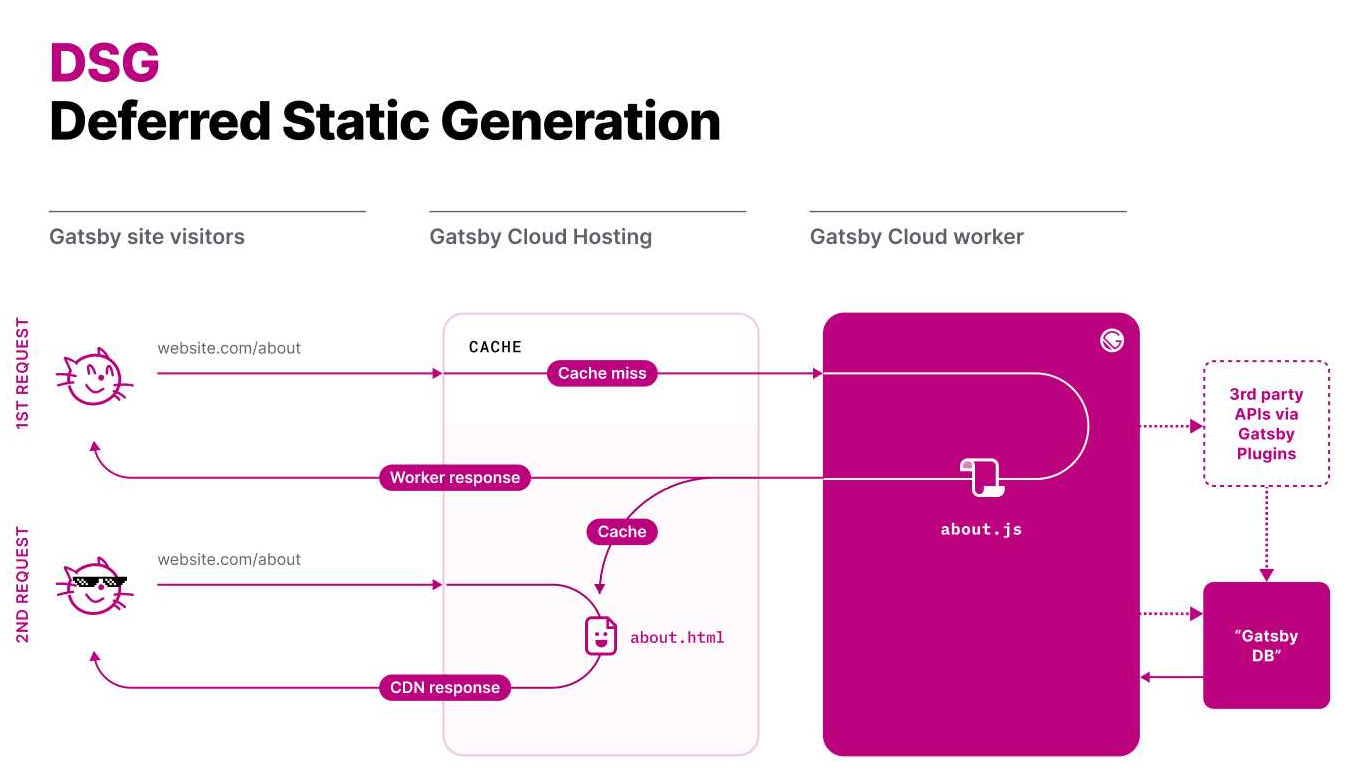
\includegraphics[width=0.9\textwidth]{media/deferred_static_generation_dsg.png}
  \legend{Fonte: \cite{gatsby2023}}
  \label{fig:deferred_dsg}
\end{figure}

Na \autoref{fig:deferred_dsg}, observa-se que, ao acessar uma página como \texttt{/about} pela primeira vez, ocorre um \textit{cache miss}, e um \textit{worker} do Gatsby é acionado para gerar o arquivo \texttt{about.html} a partir do componente correspondente (\texttt{about.js}). Esse conteúdo pode incluir dados extraídos de plugins, \textit{APIs} de terceiros ou do próprio \textit{Gatsby DB}. Após o processamento, a resposta é enviada ao usuário e armazenada em cache. Requisições futuras à mesma rota são atendidas diretamente pela CDN, com desempenho semelhante ao de páginas \acrshort{ssg}.

Segundo \citeonline{locofy2024}, a estratégia do \acrshort{dsg} é especialmente útil para projetos com milhares de páginas cujo acesso é desigual. Exemplos incluem catálogos de produtos legados, páginas de arquivos antigos ou conteúdos gerados a partir de sistemas CMS.

A seguir, um exemplo de configuração de uma rota com \acrshort{dsg} em Gatsby:

\begin{codigo}[H]
  \begin{lstlisting}[language=JavaScript]
// gatsby-node.js
exports.createPages = async ({ actions }) => {
  const { createPage } = actions
  createPage({
    path: `/produto/exemplo`,
    component: require.resolve(`./src/templates/produto.js`),
    context: { id: `produto-exemplo` },
    defer: true, // ativa DSG
  })
}
  \end{lstlisting}
  \caption{Exemplo de definição de página DSG no Gatsby}
  \label{cod:dsg_example}
\end{codigo}

Assim como o \acrshort{isr}, o \acrshort{dsg} busca combinar desempenho, escalabilidade e atualizações eficientes. No entanto, sua particularidade está em adiar completamente o custo da renderização até o momento da primeira requisição, tornando-o ideal em contextos onde o tempo de build precisa ser otimizado sem prejudicar a entrega do conteúdo a longo prazo.























\section{Frameworks Web}
\label{sec:frameworks-web}

O uso de bibliotecas e frameworks no desenvolvimento web moderno proporciona ganhos significativos de produtividade, desempenho e organização de código. Eles abstraem operações complexas e oferecem estruturas padronizadas para construção de aplicações escaláveis. A escolha da ferramenta está diretamente relacionada à abordagem de renderização adotada, seja no lado do cliente (\acrshort{csr}) ou do servidor (\acrshort{ssr}).

\subsection{Bibliotecas JavaScript}
\label{subsec:bibliotecas-js}

Bibliotecas JavaScript são conjuntos de funcionalidades reutilizáveis que fornecem recursos específicos para o desenvolvimento de aplicações web. Elas diferem dos frameworks por não imporem uma estrutura rígida, oferecendo maior flexibilidade ao desenvolvedor. A seguir, são apresentadas algumas das bibliotecas mais relevantes no contexto de renderização do lado do cliente (\acrshort{csr}):


\begin{itemize}
  \item \textbf{React:} Desenvolvida pelo Facebook, React é uma biblioteca declarativa focada na construção de interfaces de usuário por meio de componentes reutilizáveis. Seu uso do \textit{virtual DOM} permite renderizações mais eficientes, tornando-a ideal para aplicações interativas com alto desempenho. Apesar de ser comumente chamada de framework, React atua apenas na camada de visualização, exigindo bibliotecas complementares para roteamento e gerenciamento de estado~\cite{react2025}.

  \item \textbf{jQuery:} Uma das bibliotecas mais populares da era inicial do JavaScript moderno, jQuery simplifica tarefas comuns como manipulação do DOM, tratamento de eventos e requisições AJAX. Embora sua popularidade tenha diminuído com o surgimento de bibliotecas mais modernas e frameworks reativos, ela ainda é amplamente utilizada em sistemas legados e aplicações de menor complexidade~\cite{jquery2023}.

  \item \textbf{Alpine.js:} Alpine.js é uma biblioteca leve e reativa voltada para a manipulação de componentes diretamente no HTML, com uma sintaxe declarativa inspirada em Vue.js. Ela é particularmente útil para adicionar interatividade a páginas estáticas ou aplicações simples, sendo uma alternativa eficiente em cenários onde o uso de bibliotecas maiores seria excessivo~\cite{alpinejs2023}.
\end{itemize}

\subsection{Frameworks para CSR}
\label{subsec:frameworks-csr}

No modelo \acrshort{csr}, a renderização da interface é realizada diretamente no navegador do usuário, após o carregamento dos arquivos JavaScript. Frameworks como os listados a seguir são amplamente utilizados para implementar essa abordagem:

\begin{itemize}
    \item \textbf{Vue.js}: framework progressivo para construção de interfaces web interativas. Seu foco está na camada de visualização, com curva de aprendizado acessível e estrutura modular~\cite{vue2025}.
    
    \item \textbf{Angular}: framework completo mantido pelo Google, baseado em TypeScript, que oferece arquitetura robusta e recursos integrados como injeção de dependência e roteamento~\cite{angular2025}.
    
    \item \textbf{Svelte}: framework que realiza a compilação dos componentes no momento do build, eliminando a necessidade de um \textit{virtual DOM}, o que reduz o tempo de carregamento e o uso de recursos do navegador~\cite{svelte2025}.
\end{itemize}

Esses frameworks tornam o desenvolvimento com \acrshort{csr} mais eficiente e sustentável, proporcionando experiências ricas ao usuário com foco em interatividade e responsividade.

\subsection{Meta-frameworks para SSR}
\label{subsec:frameworks-ssr}

Para aplicações com foco em renderização no lado do servidor, os \emph{meta-frameworks} oferecem soluções completas, otimizando tanto o desempenho inicial quanto a indexabilidade em mecanismos de busca. Eles operam sobre frameworks tradicionais (como Vue ou Svelte) ou bibliotecas (como React), incorporando funcionalidades essenciais como roteamento, pré-renderização, recuperação de dados e \textit{hydration}.

\begin{itemize}
    \item \textbf{Next.js}: baseado em React, fornece recursos para \acrshort{ssr}, geração de sites estáticos e suporte a APIs integradas~\cite{nextjs2024}.
    
    \item \textbf{Nuxt.js}: extensão do Vue.js que oferece SSR, geração estática e arquitetura modular~\cite{nuxtjs2024}.
    
    \item \textbf{SvelteKit}: baseado em Svelte, permite renderização no servidor e no cliente, com foco em simplicidade e desempenho~\cite{sveltekit2024}.
    
    \item \textbf{Angular Universal}: solução oficial para SSR em Angular, melhora a indexação e o tempo de carregamento inicial~\cite{angularuniversal2024}.
    
    \item \textbf{Remix}: framework full-stack para React que adota um modelo de dados centrado em carregadores e ações~\cite{remix2024}.
    
    \item \textbf{Astro}: framework moderno que carrega apenas o JavaScript necessário, permitindo uso híbrido de componentes React, Vue, Svelte e outros~\cite{astro2024}.
    
    \item \textbf{Qwik}: introduz o conceito de aplicações \textit{resumíveis}, com SSR e carregamento progressivo de interatividade~\cite{qwik2024}.
\end{itemize}

Esses meta-frameworks são especialmente indicados para aplicações que priorizam SEO, acessibilidade e desempenho no primeiro carregamento, como páginas institucionais, lojas virtuais e blogs.

\subsection{Comparativo entre Frameworks CSR e SSR}
\label{subsec:comparativo-frameworks}

\begin{table}[H]
\centering
\caption{Comparação entre frameworks para CSR e SSR}
\label{tab:comparativo-frameworks}
\begin{tabular}{|p{3cm}|p{5.5cm}|p{5.5cm}|}
\hline
\textbf{Critério} & \textbf{Frameworks CSR (Vue, Angular, Svelte)} & \textbf{Meta-frameworks SSR (Next.js, Nuxt, SvelteKit, etc.)} \\
\hline
\textbf{Renderização Inicial} & O conteúdo é montado no navegador após o carregamento do JavaScript & O conteúdo é gerado no servidor e entregue já renderizado ao navegador \\
\hline
\textbf{Tempo de Carregamento} & Maior tempo de carregamento inicial (dependente do JS) & Melhor desempenho no carregamento inicial (TTFB menor) \\
\hline
\textbf{SEO} & Pode ser limitado, pois bots podem não processar JavaScript adequadamente & Excelente, já que o HTML completo está disponível para rastreadores \\
\hline
\textbf{Interatividade} & Alta, com foco em aplicações ricas e dinâmicas & Boa, com necessidade de \textit{hydration} após o carregamento \\
\hline
\textbf{Complexidade de Infraestrutura} & Menor, geralmente servido por CDNs e arquivos estáticos & Maior, exige servidores para processar cada requisição \\
\hline
\textbf{Casos de Uso Ideais} & SPAs, dashboards, aplicações com muitas interações em tempo real & Landing pages, blogs, e-commerces, sites que dependem de SEO \\
\hline
\end{tabular}
\end{table}


% \subsection{Modelos de Arquitetura Web}
% \label{subsec:modelos-arq-web}
% Os modelos arquiteturais variam conforme os requisitos de escalabilidade, manutenção e desempenho:

% \begin{itemize}
%     \item \textbf{Arquitetura Monolítica}: Um único projeto concentra \textit{frontend} e \textit{backend}, frequentemente usando \acrshort{ssr}. Possui inicialização simples, mas pode tornar-se complexo de manter e escalar.
%     \item \textbf{Microserviços}: Divide a aplicação em múltiplos serviços independentes. Cada serviço pode escolher a melhor abordagem de renderização (SSR ou CSR), facilitando a escalabilidade seletiva.
%     \item \textbf{Serverless}: As funções são executadas sob demanda em plataformas de nuvem, onde a renderização pode ocorrer tanto no servidor (funções que retornam HTML) quanto no cliente (ao entregar apenas APIs).
% \end{itemize}

% \subsection{Ferramentas e \textit{Frameworks}}
% \label{subsec:ferramentas-frameworks}
% O ecossistema de desenvolvimento web oferece diversas ferramentas que simplificam \acrshort{ssr} e \acrshort{csr}:

% \begin{itemize}
%     \item \textbf{\acrshort{ssr}}: \textit{Next.js} (React), \textit{Nuxt.js} (Vue), \textit{SvelteKit} (Svelte), entre outros.
%     \item \textbf{\acrshort{csr}}: React, Vue.js, Angular e muitas bibliotecas voltadas para \textit{Single Page Applications} (SPA).
% \end{itemize}


% \section{Infraestrutura de Serviço Web}
% \label{sec:infraestrutura-web}

% A decisão por \acrshort{ssr} ou \acrshort{csr} influencia diretamente a infraestrutura necessária:

% \begin{itemize}
%     \item \textbf{Servidores e Processamento}: Em \acrshort{ssr}, o servidor gera páginas dinamicamente, aumentando a carga de CPU. Já em \acrshort{csr}, o servidor atua mais como um provedor de arquivos estáticos e APIs.
%     \item \textbf{\english{Content Delivery Networks} (CDNs)}: Tanto para SSR quanto para CSR, uma CDN pode melhorar a distribuição de arquivos estáticos (HTML, CSS, JavaScript, imagens) e reduzir a latência.
%     \item \textbf{Escalabilidade}: Aplicações com alto número de requisições precisam de estratégias adequadas para lidar com picos de acesso. Em \acrshort{ssr}, muitas requisições simultâneas podem sobrecarregar o servidor; em \acrshort{csr}, o foco está em serviços de dados e na entrega eficiente de arquivos iniciais.
% \end{itemize}

% \textbf{Segurança} também se faz presente em ambas as abordagens. Boas práticas incluem:
% \begin{itemize}
%     \item Uso de \textbf{HTTPS} para proteger a comunicação.
%     \item Implementação de \textbf{CORS} (Cross-Origin Resource Sharing) quando necessário.
%     \item Tratamento de \textbf{tokens de sessão/autenticação} com cuidado para evitar vazamento de dados.
% \end{itemize}

% ---

\section{Experiência do Usuário}
\label{sec:ux}
A \acrfull{ux} é um aspecto crítico no desenvolvimento de aplicações web, influenciando diretamente a satisfação e a eficácia da interação do usuário com o sistema \cite{atori2023}. Para alcançar uma \acrshort{ux} satisfatória, a escolha entre \acrshort{csr} e \acrshort{ssr} deve considerar fatores como: {\acrshort{seo}}, velocidade de carregamento, interatividade e acessibilidade.
Conforme \citeonline{atori2024}, a \acrshort{ux} vai além da interface gráfica, englobando toda a jornada do usuário desde a navegação até a conclusão de tarefas. 

\subsection{\english{Search Engine Optimization} (SEO)}
\label{sec:seo}

O \acrfull{seo} consiste em um conjunto integrado de práticas de otimização, tanto no aspecto técnico quanto no de conteúdo, com três objetivos principais: maximizar a visibilidade orgânica nos mecanismos de busca, posicionar estrategicamente páginas-chave e garantir uma experiência de usuário qualificada durante o processo de busca. Essas práticas são essenciais para garantir que o conteúdo de um site seja facilmente encontrado e indexado pelos motores de busca, aumentando a probabilidade de atrair visitantes qualificados. Entre os fatores mais conhecidos, destaca-se a velocidade de carregamento da página, que impacta diretamente a experiência do usuário e a classificação nos resultados de busca \cite{conor2022}.
\begin{figure}[H]
    \centering
    \caption{Tempo de Rastreamento e Posicionamento da Página}
    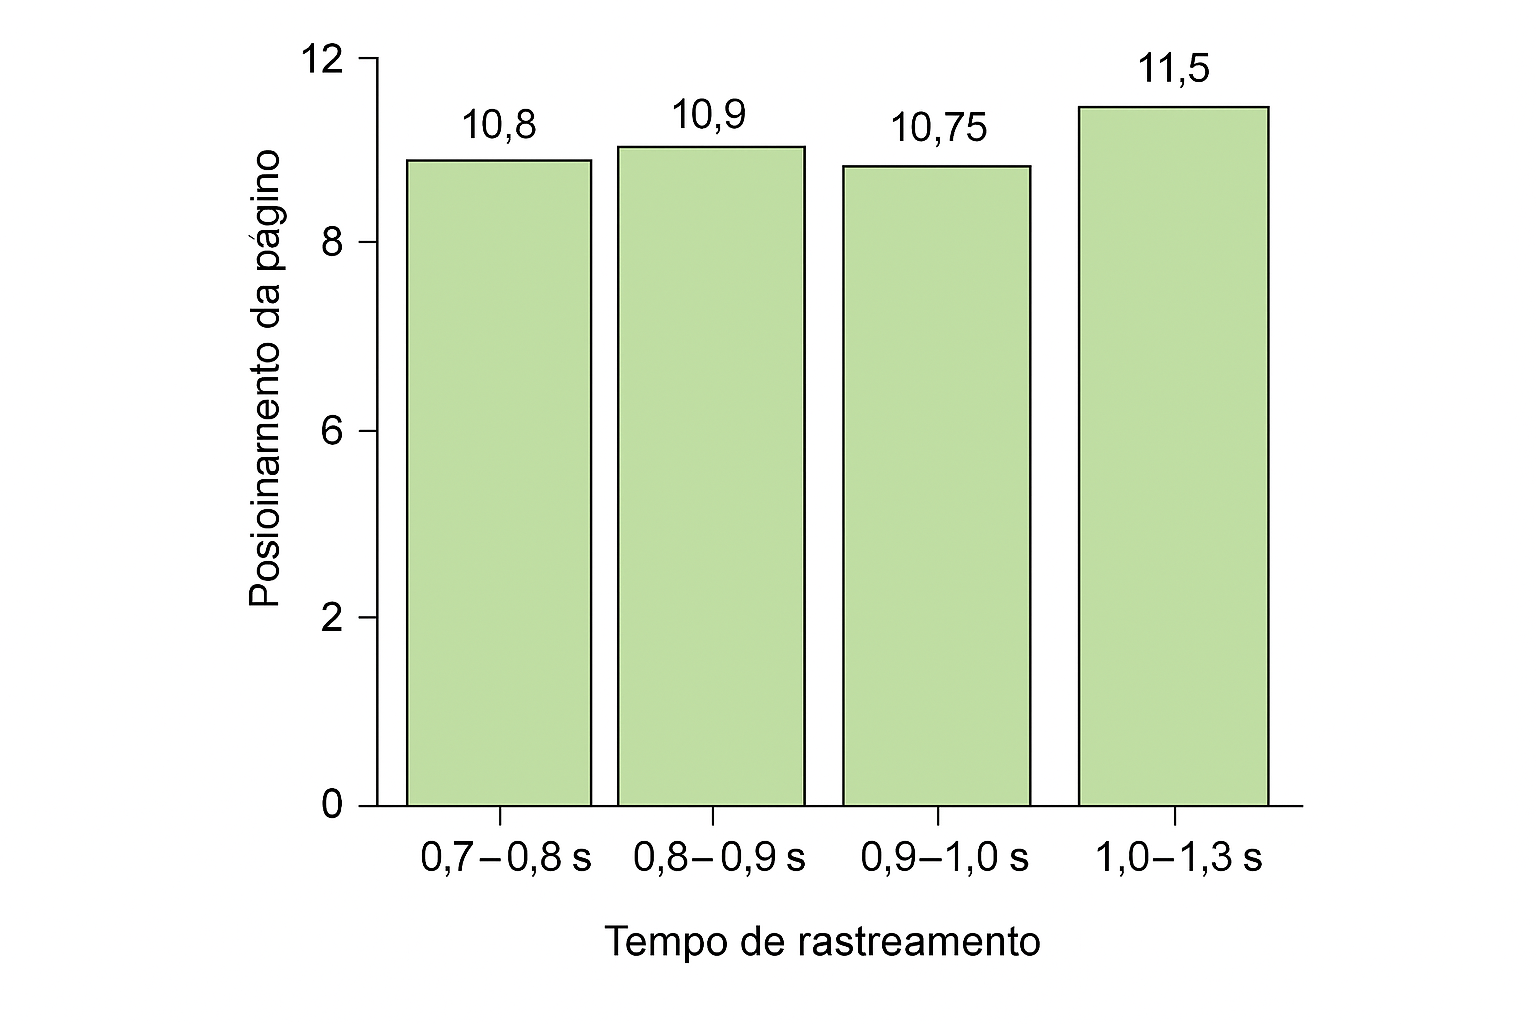
\includegraphics[width=0.6\textwidth]{media/rank_crawl_and_page_rank.png}
    \legend{Fonte: \cite{webPerformance}(adaptado)}
    \label{fig:rank_crawl_and_page_rank}
\end{figure}

A \autoref{fig:rank_crawl_and_page_rank} ilustra a relação entre o tempo de rastreamento e o posicionamento da página. O tempo de rastreamento refere-se ao tempo que os mecanismos de busca levam para acessar e indexar uma página. Quanto mais rápido o tempo de rastreamento, maior a probabilidade de a página ser indexada rapidamente e, consequentemente, melhor seu posicionamento nos resultados de busca. Isso destaca a importância de otimizar o desempenho do site para garantir uma boa classificação nos motores de busca.

\subsection{\english{Velocidade de carregamento}}
\label{sec:velocidade da página}

A velocidade de carregamento de uma página refere-se ao tempo necessário para que todo o seu conteúdo esteja visível e interativo no navegador, desde a solicitação inicial do usuário. Esse tempo pode ser influenciado por diversos fatores, como o tamanho dos arquivos, a complexidade do conteúdo, a qualidade da conexão com a internet e o desempenho do servidor \cite{shopify2024}.

Esse fator é determinante tanto para a \acrshort{ux} quanto para o \acrshort{seo}. Páginas que carregam rapidamente tendem a apresentar menores taxas de rejeição e melhores resultados em métricas de conversão. Além disso, o \acrshort{seo} utiliza a velocidade de carregamento como um dos critérios de ranqueamento nos mecanismos de busca \cite{conor2022}.

De acordo com \citeonline{google}, quanto mais rápido um site carregar, melhor tende a ser a experiência do usuário. Sites lentos comprometem a navegação e reduzem o tempo de permanência, afetando negativamente o engajamento.

A percepção de desempenho muitas vezes chamada de \emph{velocidade percebida} também é um fator crucial para a usabilidade e pode ser tão relevante quanto o tempo de carregamento real. Nesse sentido, a escolha entre \acrshort{ssr} e \acrshort{csr} influencia diretamente essa percepção. O \acrshort{ssr} geralmente proporciona carregamento inicial mais rápido, pois o conteúdo é renderizado no servidor e entregue ao navegador já pronto para exibição. Isso permite que os usuários visualizem o conteúdo principal imediatamente, mesmo que outros recursos ainda estejam sendo carregados \cite{atori2024}.

Por outro lado, no \acrshort{csr}, o navegador precisa baixar, interpretar e executar o JavaScript antes de renderizar qualquer conteúdo. Isso pode resultar em uma exibição inicial em branco ou em telas de carregamento, o que compromete a percepção de desempenho especialmente em conexões lentas ou dispositivos com menor capacidade de processamento \cite{pixelfree2023}.


\subsection{Interatividade}
\label{subsec:interatividade}

A interatividade é um fator decisivo na experiência do usuário em aplicações web modernas, pois determina a forma como os usuários percebem a continuidade e a capacidade de resposta durante a navegação. Nas aplicações que utilizam \acrshort{csr}, o código JavaScript é executado diretamente no navegador, permitindo respostas imediatas a interações como cliques, preenchimento de formulários ou navegação entre páginas internas. Essa abordagem possibilita transições de página mais suaves e experiências semelhantes às de aplicativos nativos, sem a necessidade de recarregamentos completos \cite{pixelfree2023}.

Segundo \citeonline{atori2024}, a renderização no lado do cliente favorece experiências altamente dinâmicas, oferecendo um nível elevado de controle sobre os elementos da interface. Em contrapartida, o \acrshort{ssr}, embora proporcione carregamento inicial mais rápido e visibilidade imediata do conteúdo, apresenta limitações em termos de interatividade. Alterações na interface em aplicações \acrshort{ssr} geralmente demandam comunicações adicionais com o servidor, o que pode comprometer a continuidade da experiência do usuário \cite{atori2024, splunk2023}.

Para mitigar essas limitações, abordagens híbridas têm sido amplamente adotadas. Nelas, o conteúdo é inicialmente renderizado no servidor e, posteriormente, reativado no cliente com JavaScript, em uma estratégia conhecida como \emph{hydration} \cite{splunk2023}. Essa técnica busca aliar os benefícios de desempenho e \acrshort{seo} do \acrshort{ssr} com a interatividade aprimorada do \acrshort{csr}.


\subsection{Acessibilidade}
\label{subsec:acessibilidade}

A acessibilidade em aplicações web refere-se à capacidade de tornar conteúdos e funcionalidades utilizáveis por pessoas com deficiência, como visual, auditiva, motora ou cognitiva. É um princípio essencial para garantir a equidade no acesso à informação e à interação digital. De acordo com \cite{pixelfree2023access}, acessibilidade diz respeito a assegurar que todos, independentemente de suas habilidades, possam acessar e interagir com o conteúdo da web. Para pessoas com deficiência, isso pode significar o uso de leitores de tela, navegação por teclado ou a dependência de outras tecnologias assistivas.

As abordagens de renderização, como \acrshort{csr} e \acrshort{ssr}, impactam diretamente a acessibilidade, especialmente na compatibilidade com essas tecnologias. Em aplicações que utilizam \acrshort{csr}, o conteúdo geralmente é carregado de forma assíncrona após a execução do JavaScript, o que pode dificultar a leitura imediata por leitores de tela que dependem de uma estrutura HTML previamente carregada para interpretar a página corretamente \cite{pixelfree2023access}. Já no \acrshort{ssr}, o conteúdo é entregue completamente no carregamento inicial, facilitando a interpretação por essas ferramentas e proporcionando uma experiência mais estável para usuários com deficiência visual \cite{atori2024}.

Além disso, em contextos com atualizações dinâmicas de conteúdo como ocorre em SPAs com \acrshort{csr} é necessário adotar práticas específicas para garantir a acessibilidade, como gerenciamento de foco, uso de alertas ARIA e atualização de leitores de tela após mudanças no DOM. Essas medidas são fundamentais para que as mudanças de visualização sejam percebidas corretamente por tecnologias assistivas, uma vez que alterações no DOM nem sempre são reconhecidas automaticamente por leitores de tela. O envio de foco a elementos interativos ou o uso de regiões ARIA ao vivo são técnicas recomendadas para anunciar mudanças de estado ao usuário \cite{sutton2018}.

Assim, embora o \acrshort{ssr} ofereça uma base naturalmente mais acessível, ambas as abordagens podem ser igualmente inclusivas quando aplicadas com atenção às diretrizes e boas práticas de acessibilidade.



\section{Ferramentas Modernas para Prototipação e Interfaces}
\label{sec:ferramentas-modernas}

Nesta seção são apresentadas duas ferramentas inovadoras utilizadas para acelerar o desenvolvimento frontend: a plataforma \textbf{v0} e a biblioteca de componentes \textbf{shadcn/ui}. Ambas representam abordagens modernas para construção de interfaces dinâmicas, acessíveis e escaláveis.

\subsection{v0}
\label{subsec:v0}

A \textbf{v0} é uma plataforma assistida por Inteligência Artificial projetada para transformar descrições em linguagem natural em aplicações web funcionais. A partir de prompts descritivos, a ferramenta gera código utilizando tecnologias modernas como React, Next.js e Tailwind CSS, permitindo prototipação rápida e iteração sobre interfaces \cite{v0_docs}. O fluxo básico inclui: escrever a ideia em texto, gerar a interface automaticamente, revisar e ajustar os elementos e exportar o código para integração no projeto.

\subsection{shadcn/ui}
\label{subsec:shadcn}

O \textbf{shadcn/ui} é uma biblioteca de componentes open source baseada em Radix UI e estilizada com Tailwind CSS. Ao contrário de bibliotecas tradicionais, os componentes do \textbf{shadcn/ui} são copiados diretamente para o projeto, oferecendo ao desenvolvedor total controle sobre o código e possibilitando personalizações profundas \cite{shadcn_docs}. Essa abordagem favorece flexibilidade e consistência visual no desenvolvimento de aplicações modernas.

\subsection{Integração entre v0 e shadcn/ui}
\label{subsec:integracao-v0-shadcn}

A integração entre \textbf{v0} e \textbf{shadcn/ui} proporciona uma experiência otimizada para geração de interfaces. Ao utilizar a plataforma \textbf{v0}, os componentes gerados são construídos com base na arquitetura do \textbf{shadcn/ui}, incluindo as práticas recomendadas de acessibilidade e estilização com Tailwind CSS \cite{v0_docs, shadcn_docs}. Essa integração permite que desenvolvedores iniciem com protótipos gerados automaticamente e, em seguida, façam ajustes diretamente no código dos componentes, mantendo um alto grau de personalização e performance. Além disso, ela favorece o uso de estratégias modernas como \acrshort{ssr} e \acrshort{csr}, oferecendo compatibilidade com frameworks como Next.js e Vite.




\section{Processo de Desenvolvimento e Controle de Gestão de Software}
\label{sec:git-github}

O desenvolvimento de aplicações web modernas exige práticas que garantam organização, rastreabilidade e colaboração eficiente entre desenvolvedores. Nesse contexto, ferramentas de controle de versão como o \textbf{Git} e plataformas de hospedagem como o \textbf{GitHub} são fundamentais para o gerenciamento do ciclo de vida do software \cite{github_official}.

\subsection{Git}
\label{subsec:git}

O \textbf{Git} é um sistema de controle de versão distribuído criado por Linus Torvalds em 2005 com o objetivo de gerenciar projetos de forma rápida e eficiente, independentemente do tamanho ou complexidade \cite{chacon_git}. Ele permite que múltiplos desenvolvedores trabalhem simultaneamente em um projeto, mantendo o histórico de alterações de forma segura e auditável.

Entre os conceitos fundamentais do Git, destacam-se:

\begin{itemize}
\item \textbf{Repositório (\textit{Repository}):} Estrutura que armazena o histórico completo do projeto, incluindo arquivos, diretórios e suas versões ao longo do tempo.
\item \textbf{Commits:} Registros de alterações no projeto. Cada commit possui um identificador único (hash) e uma mensagem descritiva \cite{chacon_git}.
\item \textbf{Branches:} Ramificações independentes do repositório que permitem o desenvolvimento paralelo de funcionalidades, correções ou experimentos sem impactar o código principal.
\item \textbf{Merge:} Integração de alterações realizadas em diferentes branches.
\item \textbf{Clone e Pull:} Operações que permitem obter uma cópia local do repositório e sincronizar com atualizações remotas.
\end{itemize}

O modelo distribuído do Git permite que cada colaborador mantenha uma cópia completa do repositório em sua máquina local, o que garante maior resiliência e independência em relação ao servidor central \cite{chacon_git}.

\subsection{GitHub}
\label{subsec:github}

O \textbf{GitHub} é uma plataforma de hospedagem de código baseada em Git, que amplia suas funcionalidades com recursos colaborativos e integração contínua \cite{github_official}. Fundada em 2008, a plataforma popularizou-se como um ambiente de colaboração para projetos de software de código aberto e privado.

Além de hospedar repositórios Git, o GitHub oferece funcionalidades como:

\begin{itemize}
\item \textbf{Issues:} Ferramenta para rastreamento de tarefas, bugs e melhorias \cite{github_official}.
\item \textbf{Pull Requests (PR):} Fluxo de revisão e integração de código, permitindo que contribuições sejam analisadas antes de serem incorporadas ao branch principal.
\item \textbf{Actions:} Automatização de processos com integração contínua (CI) e entrega contínua (CD).
\item \textbf{Wikis e Documentação:} Área para criação de páginas informativas sobre o projeto.
\end{itemize}

\subsection{GitHub Projects}
\label{subsec:github-projects}

O \textbf{GitHub Projects} é uma funcionalidade integrada à plataforma que possibilita o gerenciamento de projetos utilizando quadros visuais baseados em metodologias ágeis, como Kanban e Scrum \cite{github_projects}. Essa ferramenta permite organizar tarefas, acompanhar o progresso e priorizar demandas de maneira colaborativa.

Entre os recursos oferecidos pelo GitHub Projects, destacam-se:

\begin{itemize}
\item \textbf{Quadros Kanban:} Visualização de tarefas em colunas (como \textit{To Do}, \textit{In Progress} e \textit{Done}), facilitando o acompanhamento do fluxo de trabalho.
\item \textbf{Automação:} Regras automáticas que movem cartões entre colunas com base em eventos, como o fechamento de issues ou merge de pull requests \cite{github_projects}.
\item \textbf{Customização:} Campos personalizados e filtros para adaptar o quadro às necessidades do projeto.
\item \textbf{Integração com Issues e Pull Requests:} Possibilidade de vincular tarefas diretamente ao código, permitindo rastreabilidade completa entre planejamento e implementação.
\end{itemize}






\section{News API}
\label{sec:news-api}

A \textbf{News API} é uma interface de programação que disponibiliza fluxos de notícias e artigos de forma estruturada, permitindo o acesso a conteúdos de mais de 150\,000 fontes jornalísticas ao redor do mundo. Seu propósito é fornecer informações publicadas em tempo real, facilitando o desenvolvimento de soluções de agregação, análise e visualização de notícias \cite{newsapi_docs}.

\subsection{Escopo e cobertura}
A plataforma oferece dois principais tipos de consulta: 

\begin{itemize}
    \item \textbf{Busca por artigos (\texttt{/everything}):} permite pesquisar notícias com base em termos, operadores booleanos, intervalos de datas, domínios específicos e critérios de ordenação, como relevância, popularidade ou data de publicação \cite{newsapi_docs}.
    \item \textbf{Manchetes principais (\texttt{/top-headlines}):} retorna as notícias mais recentes, com filtros por país, categoria jornalística e fontes específicas.
\end{itemize}

Além disso, a \textbf{News API} disponibiliza o endpoint \texttt{/sources}, que fornece metadados sobre os veículos indexados, como nome, idioma, categoria e URL oficial.

\subsection{Autenticação e formato de resposta}
Para utilizar os endpoints, é necessário um \acrshort{api} key, que autentica as requisições e controla o uso da plataforma. As respostas são retornadas no formato \acrshort{json}, contendo campos como \texttt{status}, \texttt{totalResults} e uma lista de objetos \texttt{articles}, com atributos como título, autor, descrição, \acrshort{url} e data de publicação \cite{newsapi_docs}.

\subsection{Funcionalidade e integração}
A \textbf{News API} suporta buscas avançadas com:

\begin{itemize}
    \item termos exatos ou operadores lógicos (\texttt{AND}, \texttt{OR}, \texttt{NOT});
    \item filtros por idioma, domínios específicos e intervalos de datas (\texttt{from}, \texttt{to});
    \item paginação e controle de volume de resultados, com limite máximo de 100 artigos por página.
\end{itemize}

Essas características permitem integração tanto em aplicações com \acrshort{csr}, que realizam chamadas diretamente do navegador após o carregamento, quanto em soluções com \acrshort{ssr}, onde as requisições são feitas na camada servidor, possibilitando que o conteúdo seja renderizado previamente antes de ser entregue ao cliente.






\section{Contêineres e Docker}
\label{cap:docker}

Este capítulo apresenta os conceitos fundamentais de contêineres e da plataforma \textbf{Docker}, incluindo sua arquitetura, objetos principais (imagens, camadas, contêineres, redes e volumes) e o processo de construção de imagens por meio do \textbf{Dockerfile}. Também são discutidas boas práticas de construção (multi-stage builds, cache, uso de \texttt{.dockerignore} e \textit{secrets}) e a integração com o estudo comparativo \acrshort{csr} x \acrshort{ssr}. \cite{docker_overview,dockerfile_ref} 

\subsection{Visão Geral da Plataforma Docker}
\label{sec:docker-overview}

O \textbf{Docker} é uma plataforma de código aberto que permite empacotar, distribuir e executar aplicações em ambientes isolados chamados \textbf{contêineres}. Esses contêineres são leves, portáveis e contêm tudo o que é necessário para executar a aplicação (bibliotecas, dependências e configurações), reduzindo a variação entre ambientes e acelerando ciclos de \acrshort{ci}/\acrshort{cd} \cite{docker_overview}. 

\subsection{Arquitetura: cliente–servidor}
\label{subsec:docker-arquitetura}

A arquitetura do Docker segue o modelo cliente–servidor: o \textbf{cliente} (\texttt{docker}) envia comandos para o \textbf{daemon} (\texttt{dockerd}), que executa as operações de \textit{build}, execução e distribuição de imagens e contêineres. A comunicação ocorre via \acrshort{api} do Docker, por \textit{Unix sockets} ou interface de rede. O \textbf{Docker Desktop} integra esses componentes e ferramentas correlatas (Compose, Kubernetes opcional, etc.) \cite{docker_overview}. 

\begin{figure}[H]
  \centering
  \caption{Arquitetura simplificada do Docker (cliente, daemon, registries e objetos).}
  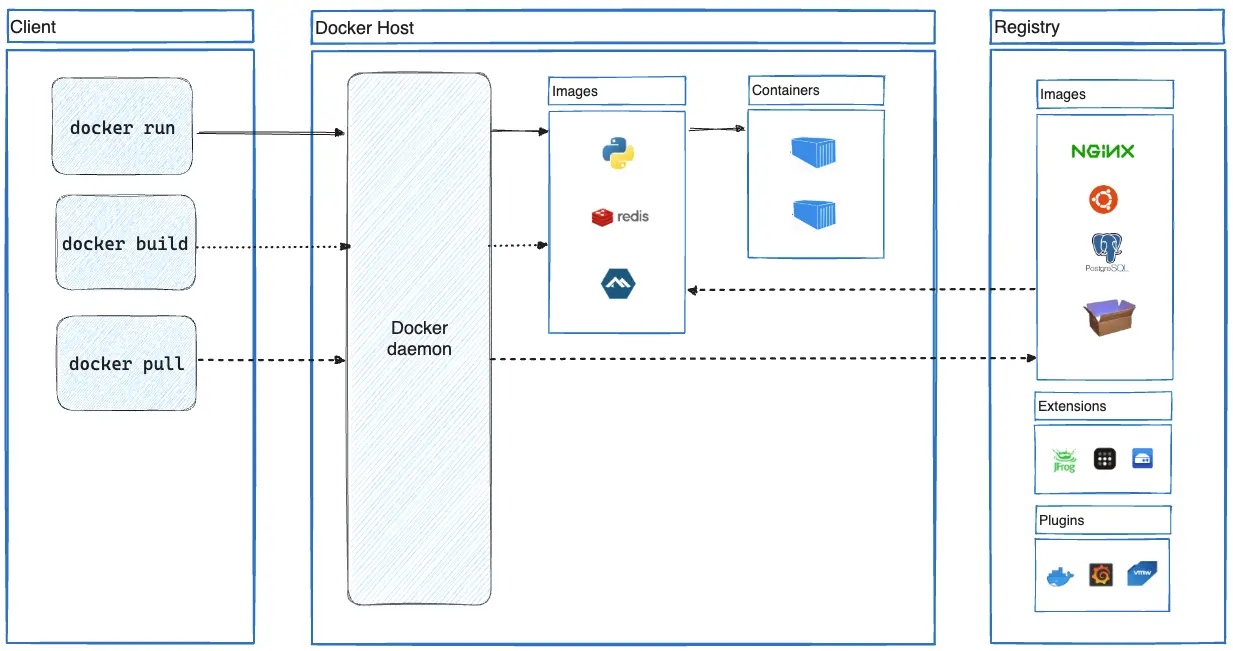
\includegraphics[width=0.8\textwidth]{media/docker_architecture.png}
  \legend{Fonte: Adaptado da documentação oficial do Docker \cite{docker_overview}.}
  \label{fig:docker-arquitetura}
\end{figure}

\subsection{Registries e distribuição de imagens}
\label{subsec:docker-registries}

Imagens são armazenadas em \textbf{registries} (Docker Hub público ou registries privados). Comandos como \texttt{docker pull}, \texttt{docker push} e \texttt{docker run} interagem com o registry configurado. Essa camada viabiliza portabilidade entre ambientes locais, datacenters e nuvens \cite{docker_overview}. 

\section{Objetos do Docker: imagens, camadas e contêineres}
\label{sec:docker-objetos}

\subsection{Imagens em camadas}
\label{subsec:docker-imagens}

Uma \textbf{imagem} é um \textit{template} somente leitura, composto por \textbf{camadas} (\textit{layers}). Cada instrução no \textbf{Dockerfile} cria uma nova camada. Em uma reconstrução, apenas camadas alteradas são recompostas, o que torna as imagens mais leves e o \textit{build} mais eficiente \cite{docker_overview}. 

\subsection{Contêineres}
\label{subsec:docker-containers}

Um \textbf{contêiner} é uma instância executável de uma imagem. Ele pode ser criado, iniciado, parado, removido e conectado a redes e volumes. Por padrão, um contêiner é isolado, mas o nível de isolamento de rede, armazenamento e \textit{namespaces} pode ser configurado. Alterações não persistentes são descartadas quando o contêiner é removido \cite{docker_overview}. 

\begin{codigo}[H]
\begin{lstlisting}[language=bash]
# Exemplo simples: criar um container Ubuntu e entrar em /bin/bash
docker run -it ubuntu /bin/bash
\end{lstlisting}
\caption{Exemplo de execução interativa de contêiner}
\label{lst:docker-run}
\end{codigo}

\section{Dockerfile: referência e instruções principais}
\label{sec:dockerfile}

O \textbf{Dockerfile} é um arquivo de texto que descreve, passo a passo, como montar uma imagem: cada instrução corresponde a um comando executado durante o \textit{build}. Entre as instruções mais comuns estão: \texttt{FROM}, \texttt{RUN}, \texttt{COPY}, \texttt{ADD}, \texttt{CMD}, \texttt{ENTRYPOINT}, \texttt{ENV}, \texttt{ARG}, \texttt{EXPOSE}, \texttt{WORKDIR}, \texttt{USER}, \texttt{VOLUME}, \texttt{HEALTHCHECK}, \texttt{LABEL} e \texttt{ONBUILD} \cite{dockerfile_ref}. 

\subsection{Formato, substituição de variáveis e \textit{.dockerignore}}
\label{subsec:dockerfile-format}

As instruções suportam formas \textit{shell} e \textit{exec} (JSON). Variáveis de ambiente podem ser interpoladas em várias instruções, respeitando o escopo e a ordem de avaliação. O arquivo \texttt{.dockerignore} exclui caminhos do contexto de \textit{build}, reduzindo tamanho de envio e prevenindo inclusão indevida de arquivos \cite{dockerfile_ref}. 

\subsection{Instruções essenciais}
\label{subsec:dockerfile-core}

\begin{itemize}
    \item \textbf{\texttt{FROM}}: define a imagem base e pode nomear estágios (\texttt{AS}). Suporta interação com \texttt{ARG} na seleção da base (por exemplo, plataforma/versão). \cite{dockerfile_ref} 
    
    \item \textbf{\texttt{RUN}}: executa comandos e compõe camadas; com BuildKit, permite \texttt{RUN --mount} para \textit{cache}, \textit{bind}, \textit{tmpfs}, \textit{secret} e \textit{ssh}, acelerando \textit{builds} e protegendo segredos. \cite{dockerfile_ref} 
    \item \textbf{\texttt{COPY}/\texttt{ADD}}: copiam arquivos do contexto; \texttt{COPY --from} permite copiar de outro estágio/imagem (\textit{multi-stage}). Flags como \texttt{--chown} e \texttt{--chmod} controlam propriedade e permissões. \cite{dockerfile_ref}
    \item \textbf{\texttt{CMD}/\texttt{ENTRYPOINT}}: definem o processo padrão; podem ser combinadas (por exemplo, \texttt{ENTRYPOINT} como executável e \texttt{CMD} como argumentos). \cite{dockerfile_ref}
    \item \textbf{\texttt{ENV}/\texttt{ARG}}: definem variáveis para \textit{build} e \textit{runtime} (sendo \texttt{ARG} não persistente na imagem final; cuidado para não vazar \textit{secrets} via \texttt{ENV}). \cite{dockerfile_ref}
    \item \textbf{\texttt{WORKDIR}/\texttt{USER}/\texttt{EXPOSE}/\texttt{VOLUME}}: definem diretório de trabalho, usuário não privilegiado, portas documentadas e pontos de montagem. \cite{dockerfile_ref}
    \item \textbf{\texttt{HEALTHCHECK}}: verifica saúde do contêiner; útil para orquestração e \acrshort{slo}s. \cite{dockerfile_ref}
\end{itemize}

\subsection{Boas Práticas de Construção}
\label{sec:docker-best-practices}

\subsection{Multi-stage builds e imagens enxutas}
\label{subsec:multi-stage}

\textbf{Multi-stage builds} permitem compilar artefatos em um estágio (com \textit{toolchains} pesadas) e copiar apenas o resultado para um estágio final mínimo (por exemplo, \texttt{alpine} ou \texttt{scratch}), reduzindo tamanho, superfície de ataque e tempo de transferência \cite{dockerfile_ref}.

\begin{codigo}[H]
\begin{lstlisting}[language=Dockerfile]
# syntax=docker/dockerfile:1
FROM node:20-alpine AS build
WORKDIR /app
COPY package*.json ./
RUN npm ci --omit=dev
COPY . .
RUN npm run build

FROM node:20-alpine AS runtime
WORKDIR /app
ENV NODE_ENV=production
# copia somente o que precisa para rodar
COPY --from=build /app/.next ./.next
COPY --from=build /app/package*.json ./
EXPOSE 3000
CMD ["node", ".next/standalone/server.js"]
\end{lstlisting}
\caption{Exemplo de multi-stage build para aplicação \acrshort{ssr} com Node/Next.js}
\label{lst:dockerfile-multistage}
\end{codigo}

\subsection{Cache de build e \texttt{RUN --mount}}
\label{subsec:cache-build}

Organize instruções do Dockerfile para maximizar \textbf{cache} (mudar menos camadas de cima). Com BuildKit, \texttt{RUN --mount=type=cache} cria caches persistentes para gerenciadores de pacotes (\texttt{apt}, \texttt{pip}, \texttt{go}) sem invalidar camadas, acelerando builds subsequentes \cite{dockerfile_ref}. 

\begin{codigo}[H]
\begin{lstlisting}[language=Dockerfile]
# syntax=docker/dockerfile:1
FROM ubuntu:24.04
RUN rm -f /etc/apt/apt.conf.d/docker-clean; \
    echo 'Binary::apt::APT::Keep-Downloaded-Packages "true";' \
    > /etc/apt/apt.conf.d/keep-cache
RUN --mount=type=cache,target=/var/cache/apt,sharing=locked \
    --mount=type=cache,target=/var/lib/apt,sharing=locked \
    apt-get update && apt-get install -y curl ca-certificates
\end{lstlisting}
\caption{Uso de cache de \texttt{apt} com BuildKit}
\label{lst:dockerfile-cache}
\end{codigo}

\subsection{\texttt{.dockerignore} e redução do contexto}
\label{subsec:dockerignore}

Use \texttt{.dockerignore} para excluir arquivos como \texttt{node\_modules}, \texttt{.git}, testes e artefatos locais. Isso reduz o contexto enviado ao daemon e evita vazamento de dados no \textit{build} \cite{dockerfile_ref}. 

\begin{codigo}[H]
\begin{lstlisting}[language=bash]
# .dockerignore (exemplo)
.git
node_modules
*.log
.env
tests/
docs/
\end{lstlisting}
\caption{Exemplo de \texttt{.dockerignore}}
\label{lst:dockerignore}
\end{codigo}

\subsection{Segredos e credenciais no build}
\label{subsec:secrets}

Evite inserir \textit{secrets} na imagem via \texttt{ENV}/\texttt{ARG}. Prefira \texttt{RUN --mount=type=secret} ou \texttt{--mount=type=ssh} para acesso temporário a chaves e tokens durante o \textit{build}. Esses valores não são gravados nas camadas finais \cite{dockerfile_ref}. 

\subsection{Rede, portas, volumes e saúde}
\label{sec:network-storage}

\textbf{Portas} podem ser documentadas com \texttt{EXPOSE}, enquanto o mapeamento real é definido em \texttt{docker run -p}. \textbf{Volumes} permitem persistência de dados; \textbf{redes} conectam múltiplos contêineres. \textbf{Healthchecks} ajudam a detectar falhas de \textit{runtime} e são úteis em composição e orquestração \cite{dockerfile_ref,docker_overview}.

\begin{codigo}[H]
\begin{lstlisting}[language=bash]
# Exemplo de execução com mapeamento de porta e volume
docker run -d --name web -p 8080:80 -v data:/var/lib/app myimage:1.0
\end{lstlisting}
\caption{Mapeamento de porta e volume em um contêiner}
\label{lst:docker-run-ports-vol}
\end{codigo}

\subsection{Fluxo de Trabalho: construir, \textit{taguear}, publicar e executar}
\label{sec:workflow}

O ciclo típico envolve: escrever o Dockerfile, \textbf{construir} (\texttt{docker build}), \textbf{taguear}, \textbf{publicar} a imagem (\texttt{docker push}) e \textbf{executar} (\texttt{docker run}). Com \textit{buildx}, pode-se produzir imagens multi-arquitetura e usar recursos avançados de cache \cite{docker_overview,dockerfile_ref}.

\begin{codigo}[H]
\begin{lstlisting}[language=bash]
# Build e tag
docker build -t ghcr.io/usuario/minhaapp:1.0 .

# Login e push no registry escolhido
docker login ghcr.io
docker push ghcr.io/usuario/minhaapp:1.0

# Execução mapeando porta
docker run -d -p 3000:3000 ghcr.io/usuario/minhaapp:1.0
\end{lstlisting}
\caption{Ciclo de construção, publicação e execução}
\label{lst:docker-workflow}
\end{codigo}

\subsection{Integração com o Estudo CSR x SSR}
\label{sec:docker-csr-ssr}

No contexto do seu trabalho, contêineres simplificam a comparação entre \acrshort{csr} e \acrshort{ssr} ao padronizar ambiente, dependências e execução:

\begin{itemize}
  \item \textbf{CSR/SSG (estático + CDN):} \textit{build} do frontend (React/Vite/Next SSG) em um estágio e \textbf{Nginx} no estágio final para servir arquivos estáticos.  
  \item \textbf{SSR (Node/Next):} multi-stage com instalação apenas das dependências de produção e \textbf{imagem enxuta} (\texttt{alpine} ou \texttt{distroless}), expondo a porta do servidor \acrshort{ssr}.
  \item \textbf{Medições reprodutíveis:} ao encapsular as variantes em imagens, é possível rodar os mesmos testes de desempenho (FCP, TTFB, INP, TTI) em hardware idêntico e com \textit{network shaping}, isolando o impacto da estratégia de renderização.
\end{itemize}

\begin{codigo}[H]
\begin{lstlisting}[language=Dockerfile]
# Nginx para app CSR/SSG (estático)
FROM nginx:1.27-alpine
COPY ./dist/ /usr/share/nginx/html
# (Opcional) Copiar nginx.conf customizado
# COPY ./nginx.conf /etc/nginx/conf.d/default.conf
EXPOSE 80
\end{lstlisting}
\caption{Servidor estático para aplicação CSR/SSG}
\label{lst:dockerfile-nginx-static}
\end{codigo}

\subsection{Síntese}
\label{sec:docker-sintese}

O Docker fornece uma base consistente para empacotar e executar aplicações, com \textbf{isolamento leve}, portabilidade e \textbf{ciclo de vida} claro (construir, distribuir, executar). O \textbf{Dockerfile} e as boas práticas descritas — \textit{multi-stage}, cache de build, \texttt{.dockerignore} e \textit{secrets} — viabilizam imagens menores, \textit{builds} mais rápidos e maior segurança. Tudo isso contribui diretamente para a reprodutibilidade e a comparabilidade dos experimentos entre \acrshort{csr} e \acrshort{ssr} \cite{docker_overview,dockerfile_ref}. 
